\documentclass{article}
\usepackage[utf8]{inputenc}
\usepackage{hyperref}
\usepackage{color}
\usepackage[a4paper, total={6in, 8in}]{geometry}
\usepackage{subcaption}
\usepackage{amsmath}
\usepackage{natbib}
\setcitestyle{authoryear,open={(},close={)}} 
\usepackage{graphicx}
\usepackage{listings} 
\lstset{language=R,
    breaklines=true,
    basicstyle=\small\ttfamily,
    stringstyle=\color{DarkGreen},
    otherkeywords={0,1,2,3,4,5,6,7,8,9},
    morekeywords={TRUE,FALSE},
    deletekeywords={data,frame,length,as,character}
}
\usepackage{cleveref}
\usepackage{amsfonts}
\usepackage{authblk}
\usepackage{lineno} 
\usepackage[nomarkers,tablesonly,nofigures]{endfloat} %figure and table to the end
\linenumbers
\renewcommand{\baselinestretch}{2.0} 
 
 
\newcommand{\source}[1]{\hfill Source: {#1}} %command definition for sources in figures
%\title{A comparison of geostatistical and non-spatial machine learning methods in $NO_2$ modelling: prediction accuracy, uncertainty quantification, and model interpretation}
\title{A comparison of spatial and non-spatial methods in statistical modelling of NO$_2$: prediction accuracy, uncertainty quantification, and model interpretation}

\author[1]{Meng Lu \thanks{Corresponding Author}}
\author[2]{Joaquin Cavieres}
\author[3]{Paula Moraga}
 

\affil[1]{Department of Geography, University of Bayreuth,
Universitaetsstrasse 30, 95447 Bayreuth, Germany

meng.lu@uni-bayreuth.de}
\affil[2]{Instituto de Estadística, Facultad de Ciencias, Universidad de Valparaíso, Valparaíso, Chile 

joaquin.cavieres@uv.cl}
\affil[3]{Computer, Electrical and Mathematical Sciences and Engineering Division, King Abdullah University of Science and Technology (KAUST), Thuwal 23955-6900, Saudi Arabia 

paula.moraga@kaust.edu.sa}
\date{}   

\begin{document}
 


%\maketitle

\newpage


\newpage
\section{Introduction}
NO$_2$ is a traffic-related air pollutant highly dynamic over space. Detailed spatial mapping of NO$_2$ is needed in health cohort studies to understand the long-term health effects of NO$_2$ on individuals. Statistical methods for NO$_2$ mapping have attracted a lot of attention with the burgeoning Machine Learning (ML)\footnote{list of abbreviations: CRPS: Continuous Ranked Probability Score; CV: Cross Validation; DF: Distributional Forest; GRF: Gaussian Random Field; GMRF: Gaussian Markov Random Field; GAMLSS: Generalised Additive Models for Location Scale and Shape; INLA: Integrated Nested Laplace Approximation; IQR: Interquartile range; GWR: Geographic Weighted Regression; KED: Kriging with external drift; LUR: Land Use Regression; MAE: Mean Absolute Error; ML: Machine Learning; RF: Random Forest; OMI: Ozone Monitoring Instrument; Quantile Random Forest; RMSE: Root Mean Squared Error; SE: stacked ensemble; SPDE: Stochastic Partial Differential Equations; Tropomi: Tropospheric monitoring instrument; UK: Universal Kriging (UK); OMI (Ozone Monitoring Instrument) VIIRS: Visible Infrared Imaging Radiometer Suite; XGB: XGBoost} methods and availability of ground monitoring station networks, atmospheric satellite products, and spatial data of our environment and atmosphere. Geospatial predictors are variables that are included as covariates in a statistical air pollution model. Four commonly-used categories of geospatial predictors of NO$_2$ are relevant to this study. First, emission-related variables, like road networks, describe where and how NO$_2$ is generated. Second, dispersion-related variables are about where NO$_2$ goes after being generated, like wind speed and direction, tell us how the emitted NO$_2$ will drift once emitted. In addition to these process-based measures, outputs from physics-based numerical models and satellite measurements of atmospheric conditions have been shown to be useful in statistical modelling of NO$_2$. Numerical models are generally very different from statistical models as they are mechanism-based simulators of a physical system. Satellite measurements do not directly reflect surface NO$_2$ concentrations, but could provide important spatial information of NO$_2$. Since August 2019, the ``Tropomi" instrument onboard the Sentinel 5p mission satellite provides the highest-resolution of NO$_2$ column density yet available, with 3.5 km by 5.5 km pixels across the satellite track.
%Commonly used geospatial predictors are air emission- (e.g. road networks) and dispersion-related (e.g. wind speed) variables, numerical modelling (e.g. with chemistry transport model) output, and atmospheric remote sensing measurements or products. A most recent (data available from Jan-2018) atmosphere sensing instrument, Tropomi (Tropospheric monitoring instrument, NSO and ESA, 2019) onboard of Sentinel 5p satellite, measures column density of a variety of gaseous air pollutants, in particular with an unprecedentedly high resolution for NO$_2$ (3.5 km x 5.5 km, across along track, since 06 August 2019). 

Statistical methods applied for spatial air pollution prediction can be broadly classified depending on whether the spatial dependency is explicitly modelled. If not modelled, we refer to the methods ``non-spatial" and otherwise ``spatial". Most of the spatial air pollution models were developed to predict at coarser resolutions, commonly 1 km or coarser \citep{young2016satellite,shaddick2018data,BELOCONI2020105578}. Non-spatial methods are more dominant in air pollution mapping, particularly in high-resolution (100 m resolution or higher) mapping. Among them, LUR (Land Use Regression) models which assume linear relationships between air pollution observations and geospatial predictors are the most studied \citep{briggs2000regression,hoek2008review}. Most recently, statistical learning \footnote{in this study, ``statistical learning" is used interchangeably with "machine learning" methods \citep{hastie2009elements}}, including regularised linear regression (e.g. Lasso and Ridge regression \citep{James2013introduction}), kernel methods such as support vector machine \citep{svm1999least}, ensemble tree-based methods such as Random Forest \citep[RF,][]{breiman2001random} and XGBoost \citep[XGB,][]{chen2016xgboost}, have been applied for feature selection or capturing the non-linear response-covariate relationships \citep{luglobal,chen2019comparison}. In air pollution mapping, several studies compared between statistical learning and conventional LUR methods  \citep{chen2019comparison,kerckhoffs2019performance,luglobal,REN2020105827,machinereview}.

Geostatistical models and Geographically Weighted Regression (GWR) are the most used spatial methods for air pollution prediction \citep{vicedo2013bayesian,li2014estimating,wang2021impacts,zou2016high} and these methods have been combined with dimension reduction \cite{zhai2018improved} and RF \citep{zhan2018satellite,liu2020integrate} to improve NO$_2$ prediction accuracy. A Bayesian geostatistical model is developed in \cite{BELOCONI2020105578} to predict NO$_2$ by integrating Tropomi satellite instrument measurements and chemical transport models. A GWR model naturally models spatial varying coefficients by fitting multiple local regressions depending on the homogeneity in response-covariate relationships when a number of observations are involved. A typical geostatistical model can be viewed as consisting of two components: a mean function, commonly a linear model, capturing the response-covariate relationships and a covariance function modelling dependency of residuals from the mean \citep{stackinla}. Conventional Kriging methods suffer from the ``big n problem", i.e. it may become computationally intractable with a large number of observations. To deal with this problem, \cite{lindgren2011explicit} propose to use Stochastic Partial Differential Equations (SPDE) to approximate the Gaussian Random Field (GRF) to a Gaussian Markov random field (GMRF, \cite{rue2005gaussian}). The main advantage of this is that the GMRF has a sparse structure of the precision matrix, which is the inverse of the covariance matrix of a GRF. Along with this, \cite{rue2009approximate} propose to use the Integrated Nested Laplace Approximation (INLA) in a Bayesian framework to achieve the computational scalability of a geostatistical model using approximations for all the estimations. This is especially advantageous when  modelling NO$_2$ over a larger scale e.g. continental or global-scale modelling when a large amount of observations are modelled, and in spatiotemporal modelling. 


%The INLA (Integrated Nested Laplace Approximation) together with SPDE (stochastic partial differential equation) \citep{lindgren2011explicit} approaches 

%approximate a spatial random field. INLA is a deterministic model and not a statistical method of optimization (e.g. as the maximum likelihood method) and it addresses the computational scalability of geostatistical methods by estimating a sparse precision matrix and using approximations for all the estimations,  

%In contrast to Geostatistical models and GWR, which identify the spatial structure based on the distance, the spatial autogressive model , which models spatial effects based on neighbourhood connections (here ground station measurements), is studied in \cite{BERTAZZON20159}.  \textcolor{blue}{(JC: I don't understand this because we don't use the neighbourhood as spatial random effect. You only are saying this as an additional comment?)}
%\textcolor{red}{PM: I agree. Maybe remove this paragraph?}
%Machine learning methods commonly have a high predictive power but lower inference capability compared to a geostatistics methods. 

As spatial models are typically more complex compared to their non-spatial counterparts, several studies compared spatial and non-spatial models to understand if the spatial effects could be simply modelled by including certain covariates in LUR models. \cite{young2016satellite} studied the use of universal Kriging (UK), OMI (Ozone Monitoring Instrument) satellite instrument \citep{OMI} and LUR models for NO$_2$ prediction at 2.5 km resolution. \cite{young2016satellite} indicated that either using UK or adding OMI in the LUR model improves a LUR model but adding OMI in a UK model only trivially improves the performance. \cite{BERTAZZON20159} shows that the inclusion of the meteorological variables accounts for spatial effects similarly to the use of spatial autoregressive models\citep{anselin2001spatial}. However, even if the spatial dependency can be captured by involving certain covariates in a LUR model, we may still need geostatistical methods to understand the spatial structure present in the data. Linear models have been used for the mean function but the relationships between NO$_2$ and predictors have been shown to be better modelled with non-linear ML methods \citep{luglobal}. Most recent studies attempt to replace the linear mean function with ML models. \cite{liu2020integrate} applied a spatial model to the residuals from an RF model for the spatial prediction of PM$_{2.5}$. \cite{stackinla} propose to stack ML models to replace the mean function in a spatial model and applied the method to disease mapping. 

Few studies have compared between geostatistical and ML models, possibly because the ML models are still relatively less studied in air pollution mapping and in the field of geostatistics. It might be more interesting to compare between geostatistical and ML  models  than geostatistical models and LUR, because ML models may be more capable of capturing the spatial dependency by integrating covariates, though implicitly, when the number of observations is sufficient. Moreover, most comparison studies only compare the Cross-Validation (CV) accuracy of the prediction mean, ignoring the confidence and prediction intervals, or the probability distributions of the parameters and predictions. If correctly derived, narrower intervals would be preferred. Also not discussed is the cause of the prediction errors, are they caused by missing covariates, violation of the model assumptions (e.g. data distribution, non-linearity), or inconsistent distributions between training and validation sets. Also, different CV strategies, e.g. how do we split the train-test sets, may lead to different model validation results. Current studies commonly ignore this problem and did not discuss the consequence of applying k-fold splitting \citep{kerckhoffs2019performance,larkin2017global,REN2020105827} or bootstrapping \citep{luglobal}. These train-test splitting methods also do not provide an indication of accuracy in spatial blocks but only at the locations of observations.
 

In this study, we focus on ensemble tree-based algorithms (e.g. RF and boosting) in the non-spatial modelling category and a hierarchical spatial model \citep{lindgren2015bayesian, blangiardo2015spatial,moraga2019} called latent Gaussian model in the spatial modelling category. Additionally, we invest in stacked models for integrating ML and  geostatistical  models. This model is treated as a spatial model and is to explore if, with ML methods to estimate the mean of a geostatistical model, it could obtain both the merits of spatial and non-spatial models. Lastly, we also developed a LUR model using Lasso as a base model for comparison.  

The uncertainty is commonly quantified by confidence intervals, or credible intervals in Bayesian inference, for the estimated parameters and by prediction intervals for the predictions from the model. If the credible intervals could be estimated, we could estimate the prediction intervals. For the methods that are used in a non-parametric setting, only the prediction intervals are quantified. For parametric models, we quantified both the prediction intervals and the confidence interval.  

Ensemble trees are nonparametric models, deriving prediction intervals is therefore less straightforward than a parametric model (e.g. a linear regression model) but has been studied and shown satisfactory results with simulated data. Prediction intervals have been most well studied for RF \citep{meinshausen2006quantile,wager2014confidence,stasinopoulos2007generalized,alakus2021rfpredinterval} and more recently for boosting \citep{duan2020ngboost,velthoen2021gradient}. Comparing probabilistic methods (i.e. prediction interval calculation) of RF and boosting is beyond the scope of this study and we focus on prediction intervals derived for RF to compare with geostatistical methods. Possibly, one of the most widely recognisable methods to derive RF prediction intervals is Quantile Random Forest (QRF) \citep{meinshausen2006quantile}. QRF has been shown to estimate middle quantiles well but may fall short at the extremes due to the limited number of observations in the tail regions \citep{velthoen2021gradient}. \cite{velthoen2021gradient} proposed to use extreme quantile regression to estimate for data outside the range of observations. Another well-recognised method is distributional regression forests (DF) \citep{schlosser2019distributional}, which embeds the GAMLSS (Generalised Additive Models for Location Scale and Shape) \citep{stasinopoulos2007generalized} into RF.  

\cite{fouedjio2019exploring} compared prediction accuracy and uncertainty quantification between KED (Kriging with external drift) and QRF by simulating data with various levels of spatial dependency. It concluded that an optimal model choice depends on the level of spatial dependency and response-covariate relationships. However, it does not account for the fact that in practice, as an ensemble tree-based method can make use of a large number of (possibly correlated) predictors without being constrained to certain (e.g. linear) relationships, the spatial dependency may be explained by the covariates despite not being explicitly modelled. 

 The objective of our study is to compare geostatistical and non-spatial ensemble tree-based models for NO$_2$ mapping, in terms of their prediction accuracy, uncertainty quantification, and model interpretation and to understand effect of modelling spatial structures. From here we will refer a geostatistical model simply as a "spatial model". More specifically, the following sub-objectives are reached:

\begin{enumerate}
    \item Optimising a set of spatial hierarchical and ML models for NO$_2$ prediction in Germany and the Netherlands.
    
    \item Developing a non-spatial and a  spatial stacked ensemble model, i.e. a stack of various ML learners.
    \item Model comparison regarding the predicted mean, prediction interval, and model interpretation.  
\end{enumerate}

    %and their potential in providing information for model improvement (indicating missing covariates).
 
%    \item Propose a framework for model comparison and spatial validation. 
    %and an optimal statistical model for high-resolution NO$_2$ mapping.
 
The spatial hierarchical model incorporates the spatial random effect along with other covariates and the estimation is performed using the R package \texttt{INLA} \citep{rue2009approximate,martins2013bayesian}. XGB, RF and Lasso are chosen for the comparison with the  spatial model and they also form the base learners in the  spatial and non-spatial stacked learning models. The ML methods are chosen for their dissimilarity. Specifically, Lasso is a linear regression model without accounting for spatial dependency. RF and XGB are non-linear models with regression trees as individual learners or algorithms of the ensemble (known as "base learners") and are not affected by dependent covariates. XGB is a highly scalable boosting method that builds tree models subsequently over the residuals of previous trees and has multiple routines to penalise model over-fitting \citep{xgboost}, which has been reported in various studies to obtain the highest prediction accuracy \cite{luglobal}. 

 
\section{Data}
NO$_2$ concentration measurements of 2017 from national ground stations of Germany (416 stations) and the Netherlands (66 stations) are used (in total: 482). The original hourly data is downloaded from the EEA \citep[European Environment Agency,][]{nelson1999european,EEA}. Negative values are considered as missing. The stations consists of  more than 25\% of missing data according to the original hourly measurements are shown in the supplementary material.  The data is aggregated to annual concentrations by taking the mean and omitting missing values. The spatial distribution of NO$_2$ stations and the station types, histogram and Q-Q plot for normality are shown in \cref{fig:histqq}. %The urban type, "rural", "suburban", and "urban" are defined respectively by the population  < 300,  301 - 1500, and > 1500, within 1 km$^2$ \citep{urbantype}.
We conducted a Shapiro test for normality, with the result implying the distribution of data being significant different from normal distribution (p-value= 8.605e-12, ``normal distribution" and ``Gaussian distribution" are used interchangeably in this study).
A Gamma distribution test was conducted using the method proposed in \cite{villasenor2015variance} and implemented in \cite{goft}.  The test result (p-value = 0.32) indicates that the data distribution is not significantly different from Gamma distribution.

\begin{figure}
    \centering
    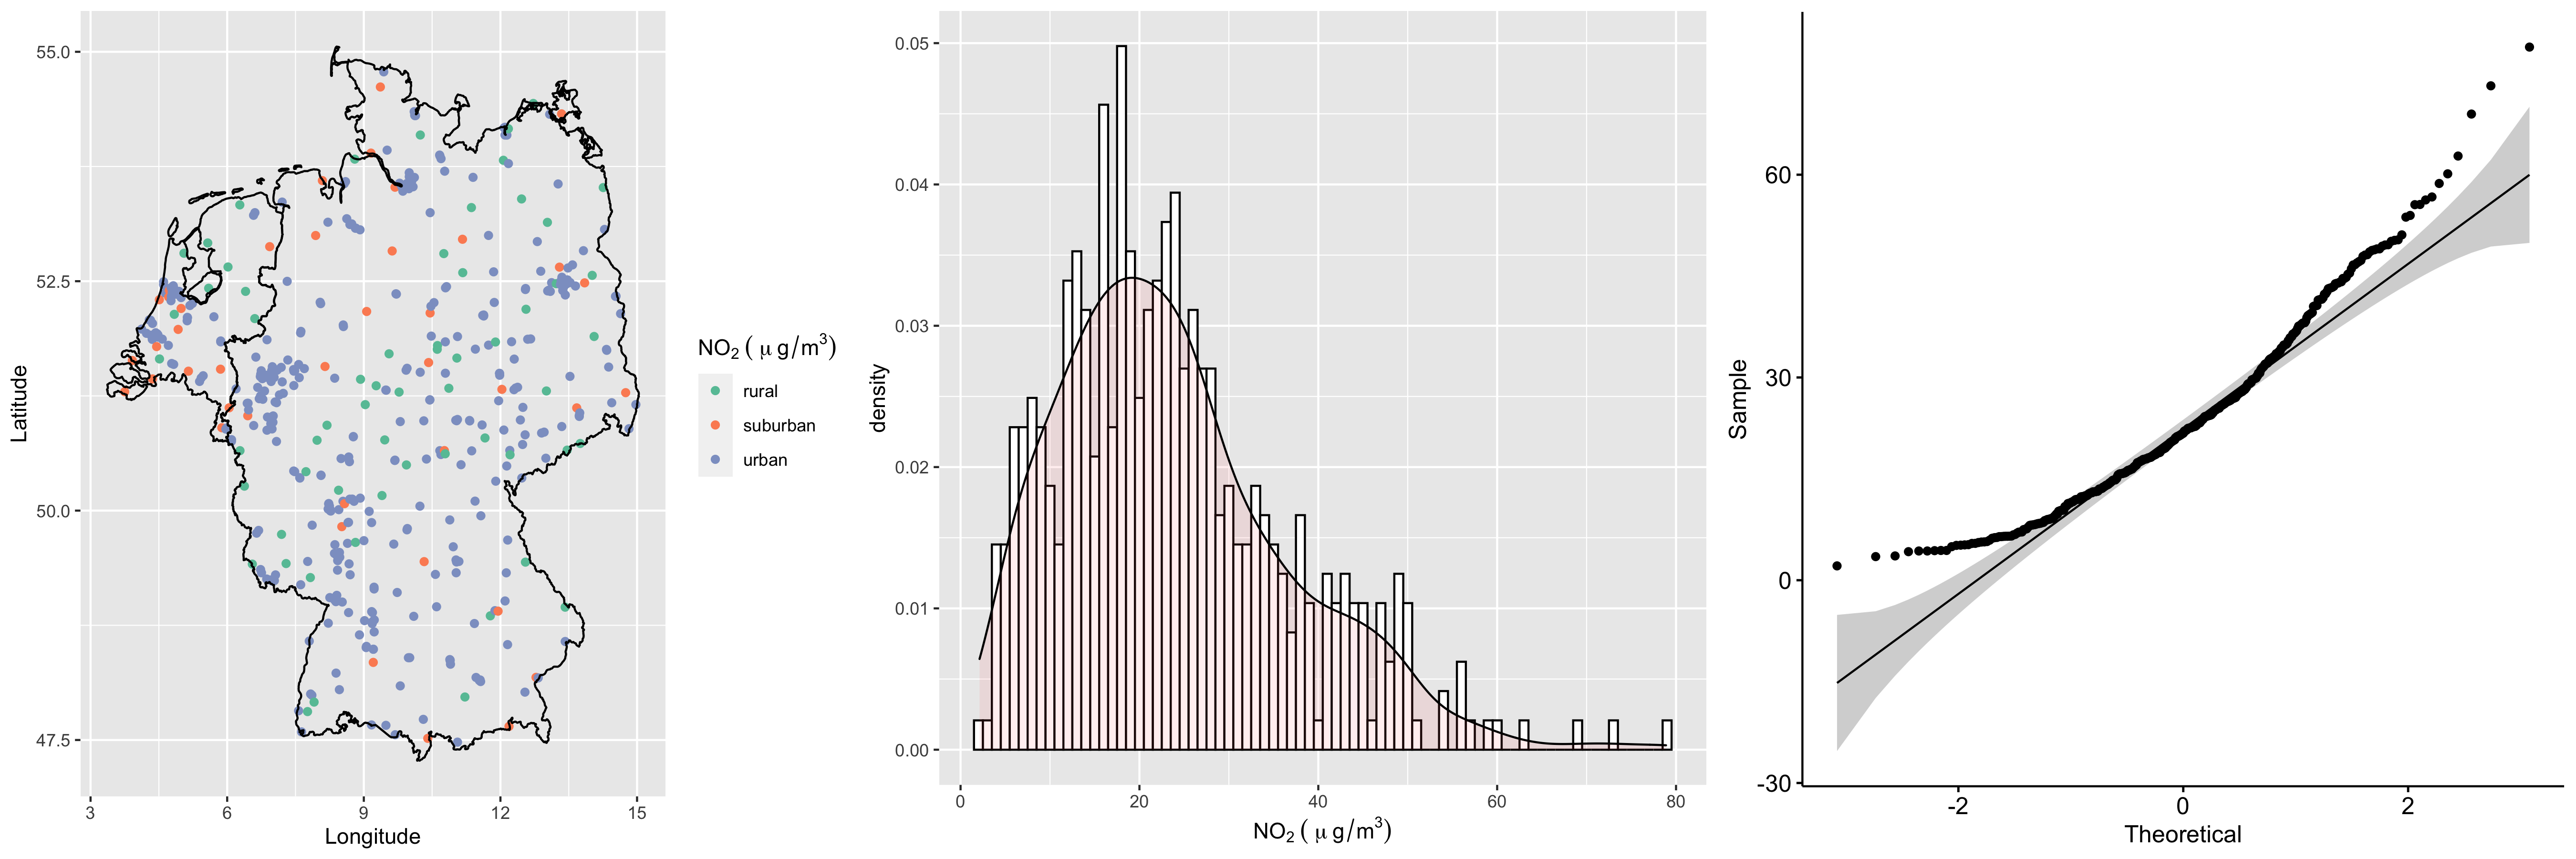
\includegraphics[scale=0.06]{fig/histqq_NO2.png}
    \caption{The geographical distribution of ground stations, histogram and Q-Q plot of the NO$_2$ measurements used in this study.}
    \label{fig:histqq}
\end{figure}{}

The geospatial predictor grids (\cref{tab:prevar}) are calculated or re-sampled at 100 m resolution. They are either spatial attributes aggregated in a circular ring centred at each sensor or prediction location, called buffered predictors, or values of the spatial attribute at the observation or prediction location, called gridded variables. The buffered predictors include total road length, total industry areas, VIIRS (Visible Infrared Imaging Radiometer Suite) nighttime day/night band radiance values \citep[nightlight,][]{nightlight} and population. Variables that are originally grids include wind speed and temperature \citep{dee2011era}, elevation \citep{elevation}, annual mean Tropomi level 3 product of NO$_2$ column density  \citep{TROPOMIgee} from 2019 (due to the increased resolution compared to 2018). The buffered predictors of road and industry are calculated from OpenStreetMap  \citep{openstreetmap}. For a detailed description of the processing of the geospatial predictors please refer to \cite{luglobal}.   
 %OMI level 3 product of the 2017 annually aggregated NO$_2$ vertical column density, and the GEOS-CHEM \citep{bey2001global,GEOS-CHEM} annual NO$_2$ surface concentration product \citep{geddes2016long} of 2013. 

 
\begin{table}[htb!] 
\centering
\caption{Geospatial predictors considered in this study. "\_mon" indicates months (mon = 1, 2....,12).  "\_buf" indicates buffer radius in meters. The road length and industrial areas are calculated with buffer radii of 100 m, 300 m, 500 m, 800 m, 1000 m, 3000 m and 5000 m. The night lights digital numbers are calculated with buffer radii of 450 m, 900 m, 3150 m and 4950 m. The original resolution is provided for gridded variables and data types for vector variables.}

\label{tab:prevar}
{
\begin{tabular}{p{4cm}|l|l|l}
\hline
Predictor                                    & Variable name                & Unit         & Resolution/data type         \\ \hline
Monthly wind speed at 10 m altitude. &  Wind\_speed\_10m\_mon   & km/hr         &    10 km \\ \hline
Monthly temperature at 2 m altitude.  & temperature\_2m\_mon  &  Celsius        &    10 km \\ \hline
%OMI 2017 annual mean vertical column density. & OMI\_mean\_filt; OMI &  $mol /cm^2$ &    0.25 arc degrees \\ \hline
 
TROPOMI 2018 mean vertical column density.  & trop\_mean\_filt; Tropomi&  $mol /cm^2$ &   0.01 arc degrees  \\ \hline

%Remote sensing product generated of 2011 from \cite{geddes2016long} & RSp &$\mu g/ m^3$ & 10 km \\ \hline
Population in 5 km grid  & population\_5000 & count  & 5 km \\ \hline
Population in 3 km grid & population\_3000 & count  & 3 km \\ \hline
Population in 1 km grid  & population\_1000 & count  & 1 km\\ \hline
Nightlight  & nightlight\_bufnl & $W cm^{-2} sr^{-1}$  & 500 m\\ \hline
Total length of highway  & road\_1\_buf  & m &polygon, lineString              \\\hline
Total length of primary roads                   & road\_2\_buf          & m  &polygon, lineString            \\\hline
Total length of local roads     & road\_M345\_buf        & m  &polygon, lineString               \\\hline
Area of industry                                    & I\_1\_buf           & m$^2$ &polygon, lineString            \\\hline
 
\end{tabular}
}  
\end{table}


\section {Methods}

The methods considered in this study are classified as spatial and non-spatial and are given the names below in this study. 

\noindent\textbf{Spatial models:}
\begin{enumerate}
\item INLA: A spatial hierarchical model fit using INLA with a Gaussian likelihood.  
\item INLA-G: A spatial hierarchical model fit using INLA with a Gamma likelihood. 
\item SE-INLA: using the spatial hierarchical model to stacked ensemble learning with Lasso, RF and XGB models as base learners;
\end{enumerate}

\noindent\textbf{Non-spatial models:}
\begin{enumerate}
%prior for NO$_2$ measurements \textcolor{red}{Model assumes priors for the different parameters. Do you mean assuming Gaussian distribution for NO$_2$ measurements?};
\item LA: A Lasso regression model; 
\item RF: A RF model; 
\item XGB: An XGB model assuming a Gaussian objective function; 
\item XGB-G: An XGB model assuming a Gamma objective function; 
\item QRFLA: using Lasso to aggregate QRF trees \citep{hastie2009elements};
\item SE: stacked ensemble learning with Lasso, RF and XGB models as base learners; 
\item QRF: quantile regression forest \citep{meinshausen2006quantile};
\item DF: distributional regression forest \citep{schlosser2019distributional}.
\end{enumerate}

To deepen our understanding of the effects of modelling the spatial process in our INLA model, we implemented an INLA model without modelling the spatial random effect (called non-spatial INLA). 

\noindent\subsection{Non-spatial methods}
Lasso is a linear regression algorithm with the L1 regularisation to shrink variable coefficients to zero, which enables "feature selection". In the cost function, the absolute value of coefficient is added to the original least squares as a penalty term. RF and XGB in this study use trees as base learners and ensemble them to reduce variability of single trees \citep{friedman2001greedy}. RF firstly randomly draws a subset of features, and then choose features from this subset to build the tree. RF \citep{breiman2001random} grows trees independently and then take the mean of the predictions of each tree. 

QRF is a non-parametric prediction interval estimation method which keeps all the observations in the terminal node for estimating the conditional probability function. Specifically, it samples from all the response values in each terminal node and use the ratio between the number of samples that is taken from each terminal node and the number of total observations in the terminal node as weights to aggregate the samples. The weights of all the trees are summed. The summed weights computed for each observation are then used to construct the empirical conditional cumulative distribution function \citep{meinshausen2006quantile}. QRFLA uses Lasso as a post-processing of QRF \citep[][page 617]{hastie2017elements}. This method firstly preserves all the trees instead of aggregating them (e.g. taking the mean of all the predictions) and then apply Lasso regression to all the trees for aggregation. This leads to a shrinkage of the tree space and theoretically reduces model variance. DF \citep{schlosser2019distributional} firstly divide data into regions as homogeneous as possible with respect to a parametric distribution, thus capturing changes in location, scale and shapes. For each tree, maximum likelihood is used to fit distributions and recursively select and split covariates according to the instability of the gradient of the likelihood at each observation along each covariate. Then, the distributional trees are ensembled for DF.

XGB is a variation of gradient boosting, which grows trees subsequently by fitting to model residuals of the previous step. XGB is scalable to multiple threads. It enables multiple penalisation paths to control model complexity to prevent model over-fitting, including regularisation (e.g. L1 regularisation) on tree width and terminal node values, as well as drop-out (dropping trees), sampling observations (take a subset of observations in each run), and early stopping (stop iterating when after a few rounds the loss does not decrease or the node does not meet the splitting rule). The default objective function for regression assumes normal distribution of target variables (and the prediction is the mean of the distribution). This assumption has been used in all the air pollution mapping studies. Here, we additionally fit a model with the objective function assuming the target variable follows a Gamma distribution (XGB-G) as the distribution of NO$_2$ measurements is closer to Gamma than normal distribution.  

Different from the ensembling in RF or XGB, SE (Stacked Ensemble) refers to a class of algorithms that trains a second-level “meta learner” to optimise the combination of a collection of base learners. The base learners are preferably diverse to capture different relationships or patterns. In this study, Lasso, RF, and XGB are the base learners. Cross-validated predicted values (commonly known as level-one data) are used to train the meta learner.  


\subsubsection{Hyperparameter setting for XGB and RF}
\label{sec:hp}

To optimise the hyperparameters of XGB, we used the grid search to optimise hyperparameters in a 5-fold CV based on the minimum RMSE (Root Mean Squared Error) and additionally manual adjustment of the hyperparameters to look at the prediction patterns. The grid search is used instead of more computationally efficient methods (e.g. Bayesian or random search) as the optimal hyperparameter range is largely known from our previous experiences \citep{luglobal,nijmegen}. The search grid for the number of iterations (nrounds) was from 200 to 3000, with a step of 200; maximum tree depth (max-depth) from 3 to 6 with a step of 1, learning rate (eta) from 0.001 to 0.1 with a step of 0.05, the penalty term Gamma \citep{xgboost} from 1 to 5 with a step of 1, the subsample is set to 0.7, L1 norm penalisation (lambda) is set to 2 and L2 norm penalisation (alpha) is set to 0. % The optimal setting for RF is minimum number of observations in the terminal node (min.node.size) equals 5 and the number of covariates to draw from all the covaraites before growing each tree (mtry) equals 12, The final setting for XGB is: nround = 3000, eta = 0.007, subsample = 0.7, max-depth = 6, Gamma =5,  lambda =2 and alpha = 0. 
For RF, we used the default setting of number of variables that are randomly drawn for each tree \citep{breiman2001random}, which is the integer part of the total number of variables divided by three. The number of trees is set to 2000 for a safe choice as the high number of trees will not negatively affect model performance. The minimum size of terminal node was optimised between 5 and 10, and was set to 5.  




\subsection{Hierarchical spatial model}

%We use a geostatistical model to predict $NO_2$ in a continuous surface.
Suppose we assume that the NO$_2$ values $y_i$ measured at locations $\boldsymbol{s_i}$, $i=1,\ldots,n$, follows a Gaussian distribution with mean $\mu_i$ and variance $\sigma^2$, where the mean $\mu_i$ is expressed as a sum of covariates and a spatially structured random effect following a zero-mean Gaussian process with a spatial covariance function \citep{moraga2019}. Assuming that NO$_2$ values are point referenced data, we can propose a statistical model for the data as:

\begin{align}
y_i & \sim N(\mu_i, \sigma^2), \hspace{3mm} i = 1, 2, \ldots, n \label{eqn:eq1}\\
\mu_i & = \boldsymbol{d_i \beta} + \boldsymbol{x}(\boldsymbol{s_i}), \label{eqn:eq2}
\end{align}
where, $\boldsymbol{d_i} = (d_{i1}, \ldots, d_{ip})$ is the vector of covariates at location $\boldsymbol{s_i}$, $\boldsymbol{\beta}=(\beta_1, \ldots, \beta_p)'$ is the coefficient vector, and $\boldsymbol{x}(\boldsymbol{s_i})$ denotes a spatial Gaussian random field. That is, $\{\boldsymbol{x}(\boldsymbol{s}_{1}),...., \boldsymbol{x}(\boldsymbol{s}_{n})\} \sim \mathcal{N}_{n}(\boldsymbol{0}, \boldsymbol{\Sigma})$, where $\mathcal{N}_{n}$ denotes a normal multivariate distribution for the spatial process specified by its mean $\mathbb{E}(\boldsymbol{x}(\boldsymbol{s}))$, and covariance function $C(\boldsymbol{s}_{1}, \boldsymbol{s}_{2}) = \text{Cov}(\boldsymbol{x}(\boldsymbol{s}_{1}), \boldsymbol{x}(\boldsymbol{s}_{2}))$. The Gaussian random field can be stationary and isotropic, where the covariance function depends only on the distance and not direction between points, that is $C(\boldsymbol{s}_{1}, \boldsymbol{s}_{2}) = \text{Cov}(\|\boldsymbol{s}_{1} - \boldsymbol{s}_{2}\|)$ and its dependence is commonly modeled using a Matérn function (\cite{stein2012interpolation, yuan2011models, diggleetal2013}). Since incorporating the spatial dependence directly with a large number of observations using a Gaussian random field is computationally expensive, \cite{rue2005gaussian} proposed the approximation of a Gaussian random field by a Gaussian Markov random field for a more efficient computational process of estimation. The main property of the Gaussian Markov random field is that it uses a conditional dependency structure through the precision matrix $\boldsymbol{Q}$. 

%This study develops two latent Gaussian models, one uses geospatial predictors as covariates and one extends from the non-spatial SE and stack the same base learners. 

%INLA is used as an individual model and for stacked modelling with RF, XGB, and Lasso as covariates. 


In this study, we compare two spatial hierarchical  models with geospatial predictors as covariates, one uses a Gaussian likelihood and the other a Gamma likelihood. The Gamma model has the same hierarchical structure as the Gaussian model: the response variable in (equation \ref{eqn:eq1}) can be represented by $y_{i} \sim \text{Gamma}(\alpha, \beta)$ where $\alpha$ is the shape parameter and $\beta$ the rate parameter. The SE-INLA model uses a Gaussian likelihood.

\subsubsection{INLA and SPDE}

To fit the  spatial models, we use the \texttt{R} package \texttt{INLA}. Following the expression proposed in (equation \ref{eqn:eq1}), the structure for the hierarchical model is: %\textcolor{blue}{(JC: I did this change to match the previous mathematical expression to the Hierarchical structure. I think that it is more appropriate to understand our spatial model in this way. The old expression is commented in overleaf.)}:

%\begin{align}
%\boldsymbol{\theta} \hspace{2mm} \sim & \hspace{2mm} \pi(\boldsymbol{\theta}) %\label{eqn:eq5}\\
%\boldsymbol{x} \mid \boldsymbol{\theta} \hspace{2mm} \sim & \hspace{2mm} %\mathcal{N}(\boldsymbol{0}, \boldsymbol{Q}(\boldsymbol{\theta})^{-1}) %\label{eqn:eq6}\\
%\eta_{i} \hspace{2mm} = & \hspace{2mm} \sum_{j}b_{ij}x_{j}\label{eqn:eq7}\\
%\boldsymbol{y} \mid \boldsymbol{x}, \boldsymbol{\theta} \hspace{2mm} \sim & %\hspace{2mm} \prod_{i \in \mathcal{I}}p(\boldsymbol{y} \mid \boldsymbol{\eta}, %\boldsymbol{\theta}) \label{eqn:eq8},
%\end{align}


\begin{align}
\mathbf{y} \mid \mathbf{x}, \theta_{1} & \sim N(\boldsymbol{D\beta} + \mathbf{A} \mathbf{x}, \theta_{1}) \label{eqn:eq3}\\
\mathbf{x} \mid \theta_{2} & \sim \mathsf{GRF}(\boldsymbol{0}, \boldsymbol{Q(\theta_{2})}^{-1}) \label{eqn:eq4}\\
\boldsymbol{\theta} & = \{\theta_{1}, \theta_{2}\},\label{eqn:eq5}
\end{align}
where $\boldsymbol{\theta}$ is the vector of hyperparameters with $\theta_{1} = \sigma^{2}$, $\theta_{2} = \{\text{log}(\tau), \text{log}(\kappa)\}$, where $\tau$ denotes the precision and $\kappa$ the range.  $\boldsymbol{x}$ is the spatial latent field, $\boldsymbol{A}$ is the projector matrix and $\boldsymbol{y}$ is the vector of the response variable $f(\cdot \mid \boldsymbol{x}, \boldsymbol{\theta})$, commonly from the exponential family of distributions. $\boldsymbol{D}$ is a covariate matrix and $\boldsymbol{\beta}$ a coefficient matrix. 

\vspace{0.2cm}

%We used "adaptive".

The \texttt{R} package \texttt{INLA} can be used to perform direct numerical calculation of the posterior distribution for a Bayesian hierarchical model (\cite{rue2009approximate}, \cite{martino2009implementing}). If we use $\boldsymbol{x}$ as a latent Gaussian field (a Gaussian Markov random field), $\boldsymbol{\theta}$ a vector of hyperparameters and $\boldsymbol{y}$ a vector of observations, assuming independent observations given the vector of the spatial latent field ($\boldsymbol{x}$) and the hyperparameters ($\boldsymbol{\theta}$), the likelihood can be expressed as:

\begin{equation} \label{eqn:eq6}
p(\boldsymbol{y}\mid \boldsymbol{x},\boldsymbol{\theta}) =\prod_{i\in \mathcal{I}} p(y_i|\eta_i,\boldsymbol{\theta}),
\end{equation}

where $\eta_{i}$ is the linear predictor and $\mathcal{I}$ contains the indices of the observed values $\boldsymbol{y}$.  

The main aim is to approximate the posterior density for the posterior of the spatial latent field and the hyperparameters. The marginal densities can be obtained:

\begin{equation} \label{eqn:eq7}
p(x_i \mid \boldsymbol{y}) = \int p(x_i \mid \boldsymbol{\theta},\boldsymbol{y})  p(\boldsymbol{\theta} \mid \boldsymbol{y}) d\boldsymbol{\theta},
\end{equation}
and
\begin{equation} \label{eqn:eq8}
p(\boldsymbol{\theta}_j|\boldsymbol{y}) = \int p(\boldsymbol{\theta} \mid \boldsymbol{y})  d\boldsymbol{\theta}_{-j}.
\end{equation}
respectively (\cite{lindgren2015bayesian, krainski2018advanced}). \\


To model data indexed in space, \cite{lindgren2011explicit} proposed a new methodology based mainly on the approximation of the Gaussian random field with the Mat\'ern function using  Stochastic Partial Differential Equations (SPDE method) as follows:

\begin{equation}\label{eqn:eq9}
(\kappa^{2} - \Delta)^{\alpha/2}(\tau(\boldsymbol{s}) x(\boldsymbol{s})) = \boldsymbol{\mathcal{W}(s)},
\end{equation}
where $\kappa$ is a scale parameter, $x(\boldsymbol{s})$ is a spatial random field, $\Delta$ is the Laplacian, $\alpha$ is the parameter that controls the smoothness of the realisations, $\tau$ controls the variance and $\boldsymbol{\mathcal{W}(s)}$  is a Gaussian spatial white noise process (\cite{lindgren2015bayesian}). For the above we can use a Gaussian Markov random field that approximates to a Gaussian random field using a triangulation of the region of study without specifying an explicit covariance structure through the SPDE method. This approximation leads to a decrease in computational burden from $\mathcal{O}(n^{3})$ to $\mathcal{O}(n^{3/2})$. 



\subsubsection{Geospatial predictor selection for the INLA model} 

As involving too many covariates (e.g. more than 12) in the INLA model brings problems in model inferencing and multicollinearity, we used Lasso to reduce the number of variables. The Lasso was used instead of ensemble tree-based methods for feature selection because it is also a linear model (same as the INLA and INLA-G models in our study). Variables are selected with the L1 norm penalty that returns a model with errors that are within one standard error of the minimum mean cross-validated error. Lasso is applied to 80\% data randomly sampled from all the observations and this process is repeated  20 times. Variables that are selected more than 90\% of the times (i.e. 18) will be considered as covariates in INLA. The times that the Lasso selected certain variables is shown in \cref{lassoselect}. The INLA modelling process applies the same bootstrapped samples for training and validation.  In addition, the AIC step-wise model selection is applied to the entire dataset to suggest a model as a further reference. The variables selected by AIC are almost the same as the Lasso selected variables, only that it does not choose the road\_class\_3\_3000, which is highly correlated with  road\_class\_1\_5000. Based on this, the road\_class\_3\_3000 is not used as a covariate in INLA.  

  \begin{table}[!htbp] \centering 
  \caption{Frequency (number of times) of variables selected by Lasso in 20 times bootstrapping and variables that are selected more than 90\% times (i.e. 18) are listed below. These variables are considered in INLA except the road\_class\_3\_3000.} 
  \label{lassoselect} 
\begin{tabular}{@{\extracolsep{5pt}} ccc} 
\\[-1.8ex]\hline 
\hline \\[-1.8ex] 
 & Variables & Frequency \\ 
\hline \\[-1.8ex] 
 1 & nightlight\_450 & $20$ \\ 
2 & population\_1000 & $20$ \\ 
3 & population\_3000 & $20$ \\ 
4 & road\_class\_1\_5000 & $20$ \\ 
5 & road\_class\_2\_100 & $20$ \\ 
6 & road\_class\_3\_300 & $20$ \\ 
7 & trop\_mean\_filt & $20$ \\ 
8 & road\_class\_3\_3000 & $19$ \\ 
9 & road\_class\_1\_100 & $18$ \\ 
%10 & road\_class\_3\_100 & $14$ \\ 
%11 & road\_class\_3\_5000 & $6$ \\ 
%12 & road\_class\_1\_300 & $5$ \\ 
%13 & road\_class\_1\_500 & $5$ \\ 
%14 & road\_class\_2\_1000 & $2$ \\ 
%15 & nightlight\_3150 & $1$ \\ 
%16 & road\_class\_2\_300 & $1$ \\ 
%17 & road\_class\_3\_1000 & $1$ \\ 
%18 & temperature\_2m\_7 & $1$ \\  
 
\hline \\[-1.8ex] 
\end{tabular} 
\end{table} 

\subsubsection{INLA model parameterisation}
The triangulated mesh constructed in the SPDE approach is shown in the supplementary  material figure. 1, with size of the inner and outer extensions around the data locations (\textit{offsets}) 1/8 of the maximum distance among all the observations for both the inner and outer extensions. The maximum allowed triangle edge lengths in the region and in the extension (\textit{max.edge }) are set to respectively 1/30 and 1/5 times maximum distance among all the observations. The Mat\'ern SPDE model is constructed with $\alpha =2$. % and  with spatial scale parameter $\kappa$ a matrix of [0, 1, 0] and variance re-scaling parameter $\tau$ a matrix [0, 0, 1].
The SE-INLA model has the same specification (i.e. mesh structure, likelihood, objective function, priors, optimisation process) as the INLA model parameterisation described above.

\section{Model evaluation}

\subsection{Cross validation}
We use RMSE, MAE (Mean Absolute Error), IQR (InterQuartile Range) and Nash-Sutcliffe model Efficiency coefficient (NSE) to assess and compare model performance. RMSE is calculated as the square root of the differences between predictions and observations; MAE is calculated as the absolute differences between predictions and observations; IQR is the differences between the third and first quartiles of the prediction. NSE is calculated as $NSE = 1- MSE / var(y)$, where MSE indicates mean squared error, var(.) indicates variance, and y indicates observed response values. %Additionally, we calculated the explained variance, $explained variance = 1- var(error) / var(y)$.  
When different data is used in CV (e.g. separating between close and far-away from roads), we additionally calculated the RRMSE (relative RMSE), RMAE (relative MAE), RIQR (relative IQR) to account for the differences in the magnitudes of response values. The RRMSE and RMAE are calculated by dividing the RMSE and MAE, respectively, by the mean of observations. The RIQR was calculated by dividing the IQR by the median of observations. The three CV methods we designed and used to assess our model performance are: 

\begin{enumerate}
\item Bootstrapped CV. 20-times randomly bootstrapped splitting of training and test sets \citep{luglobal}.  

 %   \item Probability sampling: higher probability is given to select observations that are isolated, to test how good the model is at predicting air pollution over the whole region. This is because with random sampling we would get more points in areas where observations are clustered and may not pick any observation in areas with few observations.   
\item Spatial-blocked CV. Dividing data into spatial blocks, each time use one block for test and other blocks for training. In this study, the spatial grids are divided with the cell size 2 degree (around 222 km), which leads to 20 spatial blocks.
    
\item Customised CV. Splitting train-test based on values of certain covariates. In this study, three sub-areas are defined, 1) close to traffic and with high population ("tr-hp"), 2) close to traffic and with middle low population ("tr-lmp"), 3) far away from traffic ("far"). High population is defined as the variable population of 1000 m buffer that is in the last quartile. Low population is defined as the variable population of 1000 m buffer is below the median. Close to road is defined as (please refer to \cref{tab:prevar} for the definition of covariates): 
the road\_class\_2\_100 is larger than 0, or the road\_class\_1\_100 is larger than 0, or the road\_class\_3\_100 is within its 75-th percentile.  
Far away from road is defined as:
the road\_class\_2\_100 is 0, and the
    road\_class\_1\_100 is 0, and the
    the road\_class\_3\_100 is below its median.  
    
     
    %\item Validation based on known attribute: we know the air quality station types (traffic, background, industrial) and human settlement types (urban or rural), this allows us to quantify prediction accuracy for each type of air quality stations and separating between urban and rural areas. 
\end{enumerate}
This yields 85, 65, and 177 samples in each category. This ensures a balanced number of samples between close to traffic and far-away from traffic. Each time, 30 samples (7\% of the entire dataset) are drawn from the corresponding category for CV. For example, each time, 30 samples are drawn from the 85 samples as the test set to obtain the prediction accuracy CV for the situation "tr-hp" and the rest is used for training.  

\subsection {Prediction intervals}
CRPS (Continuous Ranked Probability Score) and coverage probabilities are used as quality indicators of prediction intervals. CRPS is an uncertainty measure that assesses the similarity between two distributions.  We use it to indicate how the predicted distribution matches the observed distribution. The CRPS implemented in the R package {\tt ScoringRules} \citep{jordan2017evaluating} is used. CRPS is calculated for the INLA and QRF models. For the INLA model, the prediction intervals are calculated by simulating from the response Y $\sim N(\theta, \sigma^2)$ where $\theta$ and $\sigma^2$ are the fitted mean and variance. The mean of CRPS for all the points within each test block is calculated in spatial-blocked CV. Coverage probabilities are calculated as the ratio between the number of predictions within the upper and lower quantile and the total number of predictions (in the test set). The prediction intervals are mainly compared between INLA, INLA-G, QRF and DF. The prediction interval for QRFLA is compared with QRF to investigate the effects of Lasso tree-aggregation strategy on the prediction intervals.
 
\subsection{Model interpretation}
%Model interpretation is compared between INLA (linear model), RF and XGBoost, as they represent linear regression, bagging and boosting. 
We inspect fixed and spatial random effects modelled by INLA and compare the spatial random field with modelled prediction intervals and model residuals to understand the contribution of spatial random effects. Different from linear regression methods, which themselves are the best models for interpretation, interpreting ensembling tree-based methods requires external models \citep{NIPS2017_8a20a862}. We use SHAP \citep[SHapley Additive exPlanations,][]{lundberg2018explainable,NIPS2017_8a20a862}, a unified method based on additive feature attribution, to estimate variable influence in RF and XGB models.   
%For a linear model like INLA, the best explanation model is the linear model itself but for ensembling methods it is harder to interpret the models \citep{NIPS2017_8a20a862}. We use SHAP \citep{NIPS2017_8a20a862} to interpret the ensemble tree models.


%\item XGboost
%Quantile regression is used to calculate the prediction quantiles of XGBoost, based on \cite{quantile} 

%\item Lasso


\section{Results}
\subsection{Accuracy assessment and uncertainty quantification}

\noindent \textbf{Spatial-blocked CV}

Spatial-blocked CV provides information about prediction accuracy in spatial blocks. 
We compare the spatial patterns of NSE as an indicator of model prediction accuracy and spatial patterns of CRPS as an indicator of the quality of the prediction intervals, of INLA, representing spatial method, and RF, representing non-spatial models. As the XGB outperforms RF in non-spatial CV, we also compares the spatial-blocked NSE for XGB. 

The NSE map (\cref{fig:r2}) shows that the XGB, RF and INLA predict relatively well in most parts of Germany besides blocks at the boundaries. The NSE for the block western the Netherlands is also relatively low with all the three methods and especially for XGB (NSE: 0.2). RF obtains the best result for the block of western the Netherlands (NSE: 0.5). The INLA model outperforms RF and XGB in the blocks at south-east and north. The NSE between blocks are the most heterogeneous with XGB, which is consistent to the result of bootstrapped CV that the XGB falls short at predicting extremes.  

The spatial-blocked CRPS \cref{fig:crps} is computed for QRF and INLA. We did not show the DF as it will be seen that the QRF and DF performed similarly in predicting the intervals (\cref{sec:predinterval})). The INLA predicted prediction distribution deviates considerably from observed distribution for the block of western the Netherlands, as reflected by the high value of mean CRPS. This is consistent to the relatively low NSE observed for the same block. However, some blocks with relatively high NSE (in the north and south) have high CRPS. This indicates that the prediction mean is well-predicted but not the prediction interval (too narrow). 

\textbf{Non-spatial CV}

Both ensemble tree-based methods with a Gaussian objective function and INLA with a Gaussian likelihood function obtain higher prediction accuracy than Lasso (\cref{cv}), indicating the necessity of using a more flexible model and modelling the spatial random fields. Among individual methods, in terms of NSE and RMSE, INLA with Gaussian likelihood obtained the highest prediction accuracy, followed by XGB and QRFLA. QRFLA greatly improves from the original RF. Despite the distribution of response being closer to Gamma distribution compared to Gaussian distribution, using Gamma regression in XGB and specifying Gamma likelihood in INLA both decrease the prediction accuracy considerably. Compared to INLA, XGB obtained lower RMSE and NSE despite it obtained lower MAE and IQR, indicating that the XGB model predicts less well at more extreme ranges. The QRF and DF results are not shown in \cref{cv} as the results are very similar to RF. Their prediction intervals are compared. 

 
SE-INLA improves prediction accuracy compared to SE and INLA, obtained the best results in terms of root mean squared error (6.83, 24.5\% of the mean of observations) and NSE (0.71). This indicates the explicit modelling of spatial structures could further improve the prediction accuracy despite flexible relationships captured from ML models.
 
\begin{table}[!htbp] \centering 
  \caption{Prediction accuracy matrix for different models using 20 times bootstrapped cross-validation. Non-spatial models: LA: Lasso; RF: random forest, XGB: XGBoost using the default Gaussian loss; XGB-G: XGBoost using a Gamma loss; QRFLA: quantile random forest with Lasso for shrinkage aggregation of regression trees; SE: stacked ensembling. Spatial models: INLA: a latent Gaussian model implemented using INLA assuming a Gaussian likelihood. INLA-G: a latent Gaussian model implemented using INLA assuming a Gamma likelihood. SE-INLA, geostatistical stacked ensembling.} 
  \label{cv} 
\begin{tabular}{@{\extracolsep{5pt}} ccccccc|ccc} 
\\[-1.8ex]\hline 
\hline \\[-1.8ex] 
         & LA  & RF   & XGB     & XGB-G & QRFLA   & SE  & INLA  &INLA-G & SE-INLA\\ 
\hline \\[-1.8ex] 
RMSE & $7.54$ & $7.45$ &$7.14$ & $8.91$ & $7.23$ &7.18& $7.06$ & 9.21 & $6.83$\\ 
IQR & $8.47$ & $7.39$ & $6.54$ & $9.21$ & $7.27$ &7.30& $7.1$ & 7.4  & $6.8$\\ 
MAE & $5.69$ & $5.51$ & $5.05$ & $6.27$ & $5.28$ &5.31& $5.3$ & 6.2  & $5.0$\\ 
 
NSE & $0.65$ & $0.65$ & $0.68$ & $0.51$ & $0.67$ & 0.69& $0.69$ &  0.45& $0.71$\\ 
\hline \\[-1.8ex] 
\end{tabular} 
\end{table} 
 

Compared to the INLA model, the non-spatial INLA model obtained lower DIC (Deviance Information Criterion, 3286.66 vs. 3251.97 with spatial effects) and WAIC (Watanabe-Akaike information criterion, 3291.75 vs. 3253.93 with spatial effects). These suggest the advantage of modelling the spatial effects. We normalised covariates before inputting into the spatial and non-spatial INLA models and compared the differences between the fixed-effects obtained by the original and non-spatial INLA model (supplementary material figure 3-4) and found the most notable change being the increased effect of the population\_1000 for the non-spatial INLA model. This can be explained by that part of the effects of population\_1000 is modelled in the spatial random field. The second most notable change is on the decreased effect of nightlight\_450 for the non-spatial INLA model. After the spatial process is modelled, the nightlight\_450 has a higher contribution to the model. Together with the decreased effects of road\_class\_2\_100 and road\_class\_3\_300 for the non-spatial INLA model, these may indicate that the spatial model could better account for traffic-related variables (i.e. road and nightlight in smaller buffers).




\begin{figure}
    \centering
    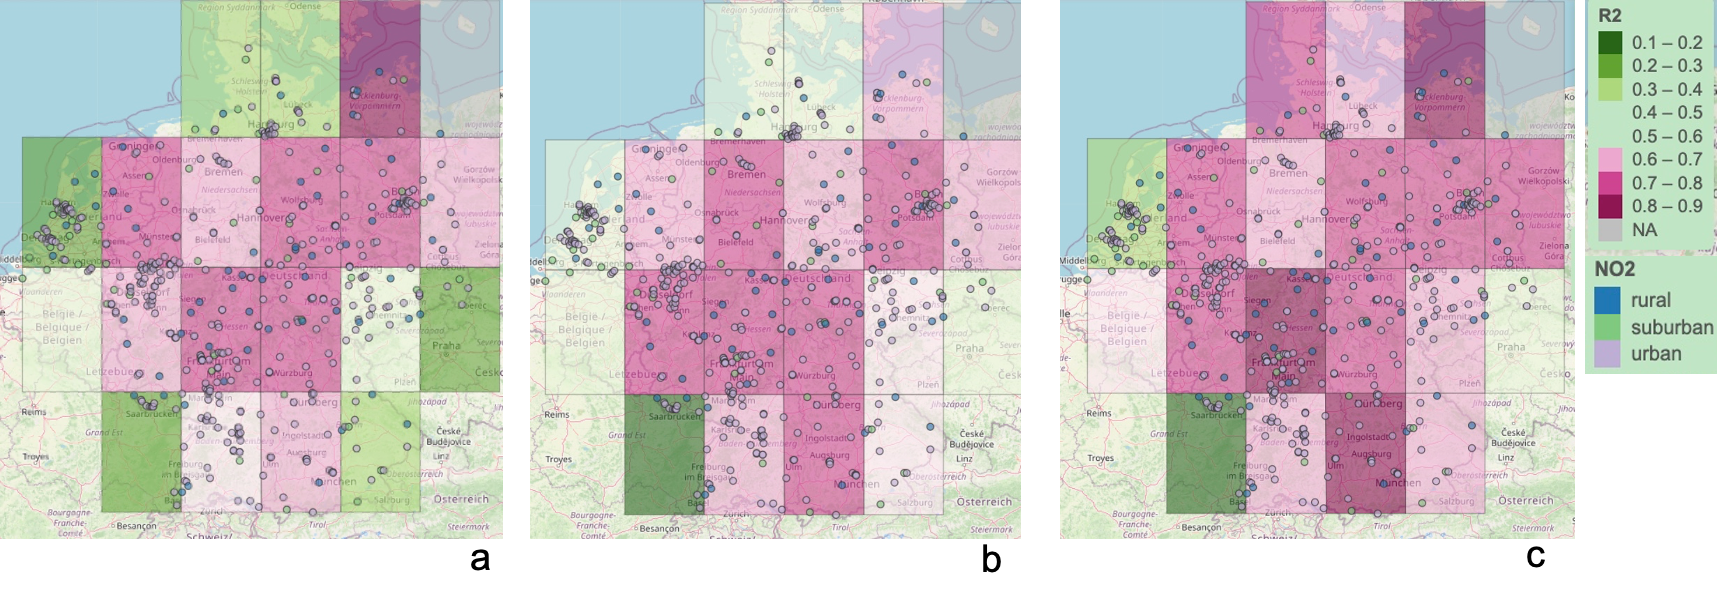
\includegraphics[scale=0.4]{fig/r2spcv.png}
    \caption{The NSE of each block, using the rest of the blocks for training. The models are a) XGB, b) QRF, c) INLA. 
}
    \label{fig:r2}
\end{figure}

\begin{figure}
    \centering
    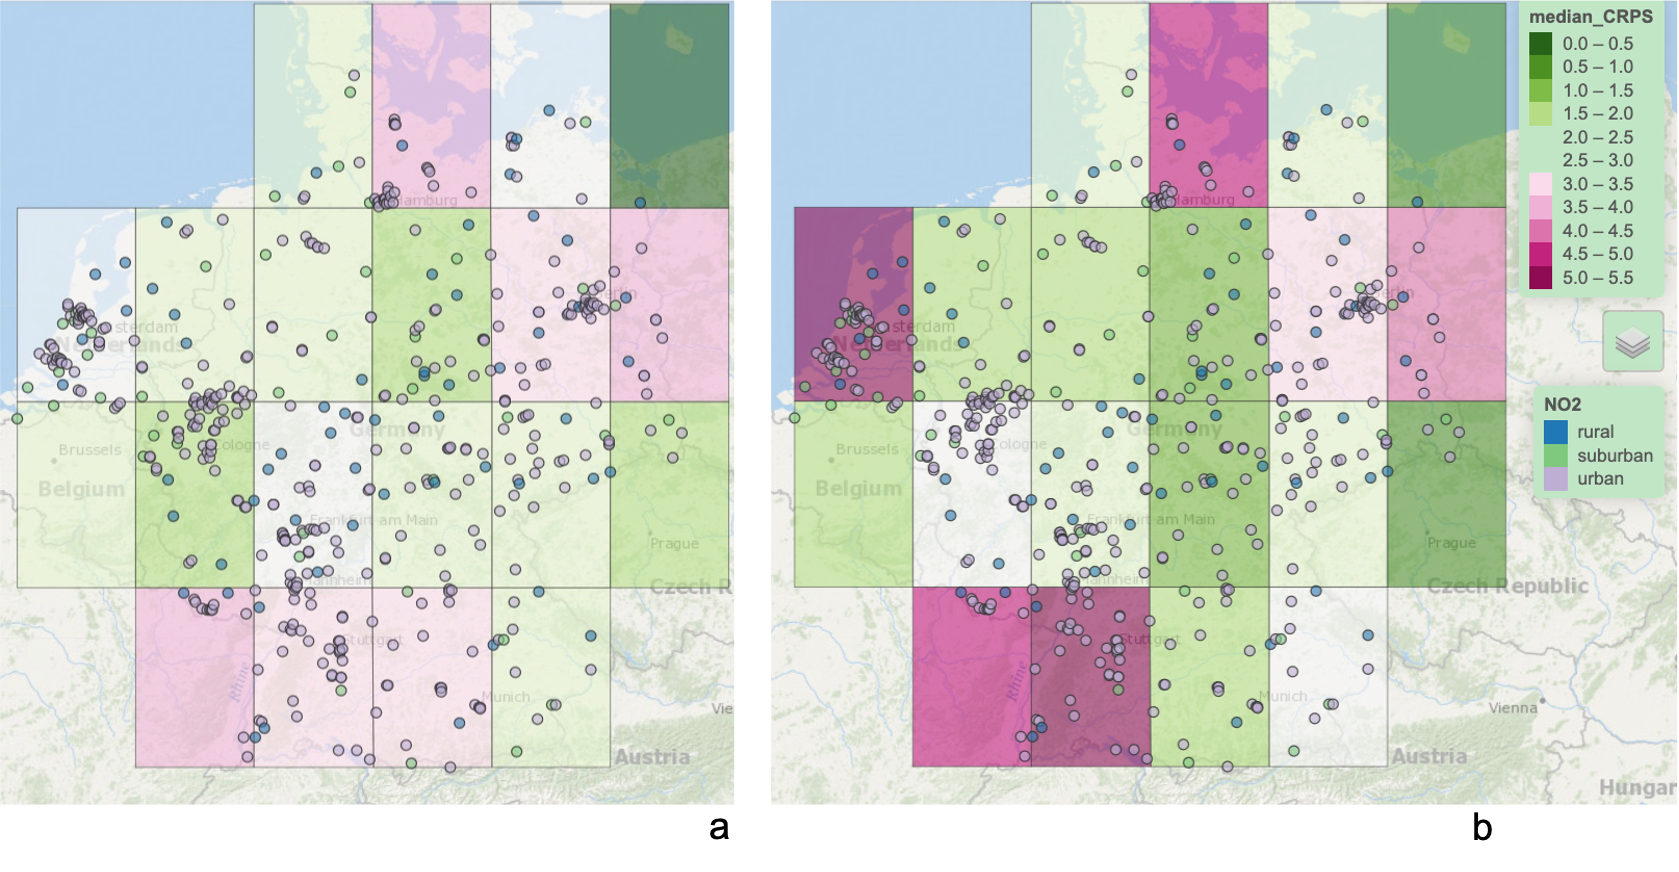
\includegraphics[scale=0.3]{fig/crps_RF_INLA.png}
    \caption{The CRPS (Continuous Ranked Probability Score) of each block, using the rest of the blocks for training. a) RF, b) INLA. 
}
    \label{fig:crps}
\end{figure}

\vspace{0.5cm}
\noindent \textbf{Customised CV}

There is a distinctive difference between model performance in areas close to traffic (i.e. \textit{tr-hp} and \textit{tr-lmp}) and far away from traffic (i.e. \textit{far}). The INLA model outperformed other non-spatial methods in both \textit{tr-hp} and \textit{tr-lmp}, especially for the latter while the XGB model outperformed the INLA model (and all the other models) in \textit{far}. This indicates the importance of modelling spatial dependency in areas close to traffic and possibly non-linear relationships far-away from roads. All the ensemble tree-based methods obtained much worse results compared to linear regression methods in \textit{tr-lmp}. A linear regression model typically outperforms ensemble tree-based methods when there are relatively few observations for a flexible relationship to be justified. As the number of observations that are close to traffic and far away from traffic is balanced, the results indicate that the population density alters relationships between NO$_2$ and road density (i.e. the relationships between NO$_2$ and road density is different with different population density) in areas close to traffic. 

\begin{table}[!htbp] \centering 
  \caption{Results with customised CV. tr-hp: close to traffic and high population, tr-lmp: close to traffic and middle and low population, far: far away from traffic. RRMSE (relative RMSE), RMAE (relative MAE), RIQR (relative IQR).} 
  \label{customisedCV} 
\begin{tabular}{@{\extracolsep{5pt}} cccccccc} 
\\[-1.8ex]\hline 
\hline \\[-1.8ex] 
 & RMSE & RRMSE & IQR & RIQR & MAE & RMAE & NSE \\ 
\hline \\[-1.8ex] 
LA\_tr-hp & $12.4$ & $0.3$ & $17.3$ & $0.4$ & $10.2$ & $0.3$ & $0.11$  \\ 
RF\_tr-hp & $11.9$ & $0.3$ & $17.8$ & $0.5$ & $9.8$ & $0.3$ & $0.18$   \\ 
XGB\_tr-hp & $11.6$ & $0.3$ & $15.3$ & $0.4$ & $9.3$ & $0.2$ & $0.21$ 
\\
INLA\_tr-hp & $11.3$ & $0.3$ & $16.6$ & $0.4$ & $9.5$ & $0.3$ & $0.26$
\\ 
\hline
LA\_tr-lmp & $7.5$ & $0.3$ & $10.4$ & $0.5$ & $6.1$ & $0.3$ & $0.21$ 
\\ 
RF\_tr-lmp & $8.2$ & $0.4$ & $10.9$ & $0.5$ & $6.4$ & $0.3$ & $0.05$  \\ 
XGB\_tr-lmp & $8.2$ & $0.4$ & $10.5$ & $0.5$ & $6.4$ & $0.3$ & $0.04$   \\ 
INLA\_tr-lmp & $6.7$ & $0.3$ & $8.7$ & $0.4$ & $5.3$ & $0.2$ & $0.36$ \\ 

\hline
LA\_far & $5.0$ & $0.4$ & $4.9$ & $0.4$ & $4.2$ & $0.3$ & $0.47$  \\ 
RF\_far & $4.9$ & $0.3$ & $4.0$ & $0.3$ & $3.6$ & $0.3$ & $0.47$  \\ 
XGB\_far & $3.4$ & $0.2$ & $3.6$ & $0.3$ & $2.5$ & $0.2$ & $0.74$   \\ 
INLA\_far & $4.0$ & $0.3$ & $4.3$ & $0.3$ & $3.2$ & $0.2$ & $0.65$

\\
\hline 
\\[-1.8ex] 
\end{tabular} 
\end{table} 




\subsection{Prediction interval}
 
After examining the quality of the prediction intervals. We compare prediction intervals estimated from RF-based methods with prediction intervals estimated in two different methods, QRF and DF (\cref{distvsquant}), RF-based method with and without Lasso postprocessing, QRF and QRFLA (\cref{qrrfla}) and the spatial models with different likelihood functions (\cref{inlapred}). 
 
The 90\% prediction intervals for INLA, INLA-G, DF, QRF and QRFLA are shown in \cref{distvsquant,inlapred,qrrfla}. The RF-based methods, namely DF, QRF and QRFLA reach the coverage probability higher than 0.9, but the DF predicts a more realistic prediction quantile, notably, it covers four observations that are not covered by the same prediction quantiles predicted by the QRF. The INLA 90\% prediction interval is too narrow. The coverage probability is 0.41 for INLA and 0.36 for INLA-G. The predicted 90-th quantile of the INLA-G turned to better capture extreme high values but miss more at the lower values. The QRFLA predicted a slightly narrower prediction interval compared to QRF. This indicates that the Lasso-based postprocessing could reduced the variance of a QRF model.  

\label{sec:predinterval}
\begin{figure}
\centering
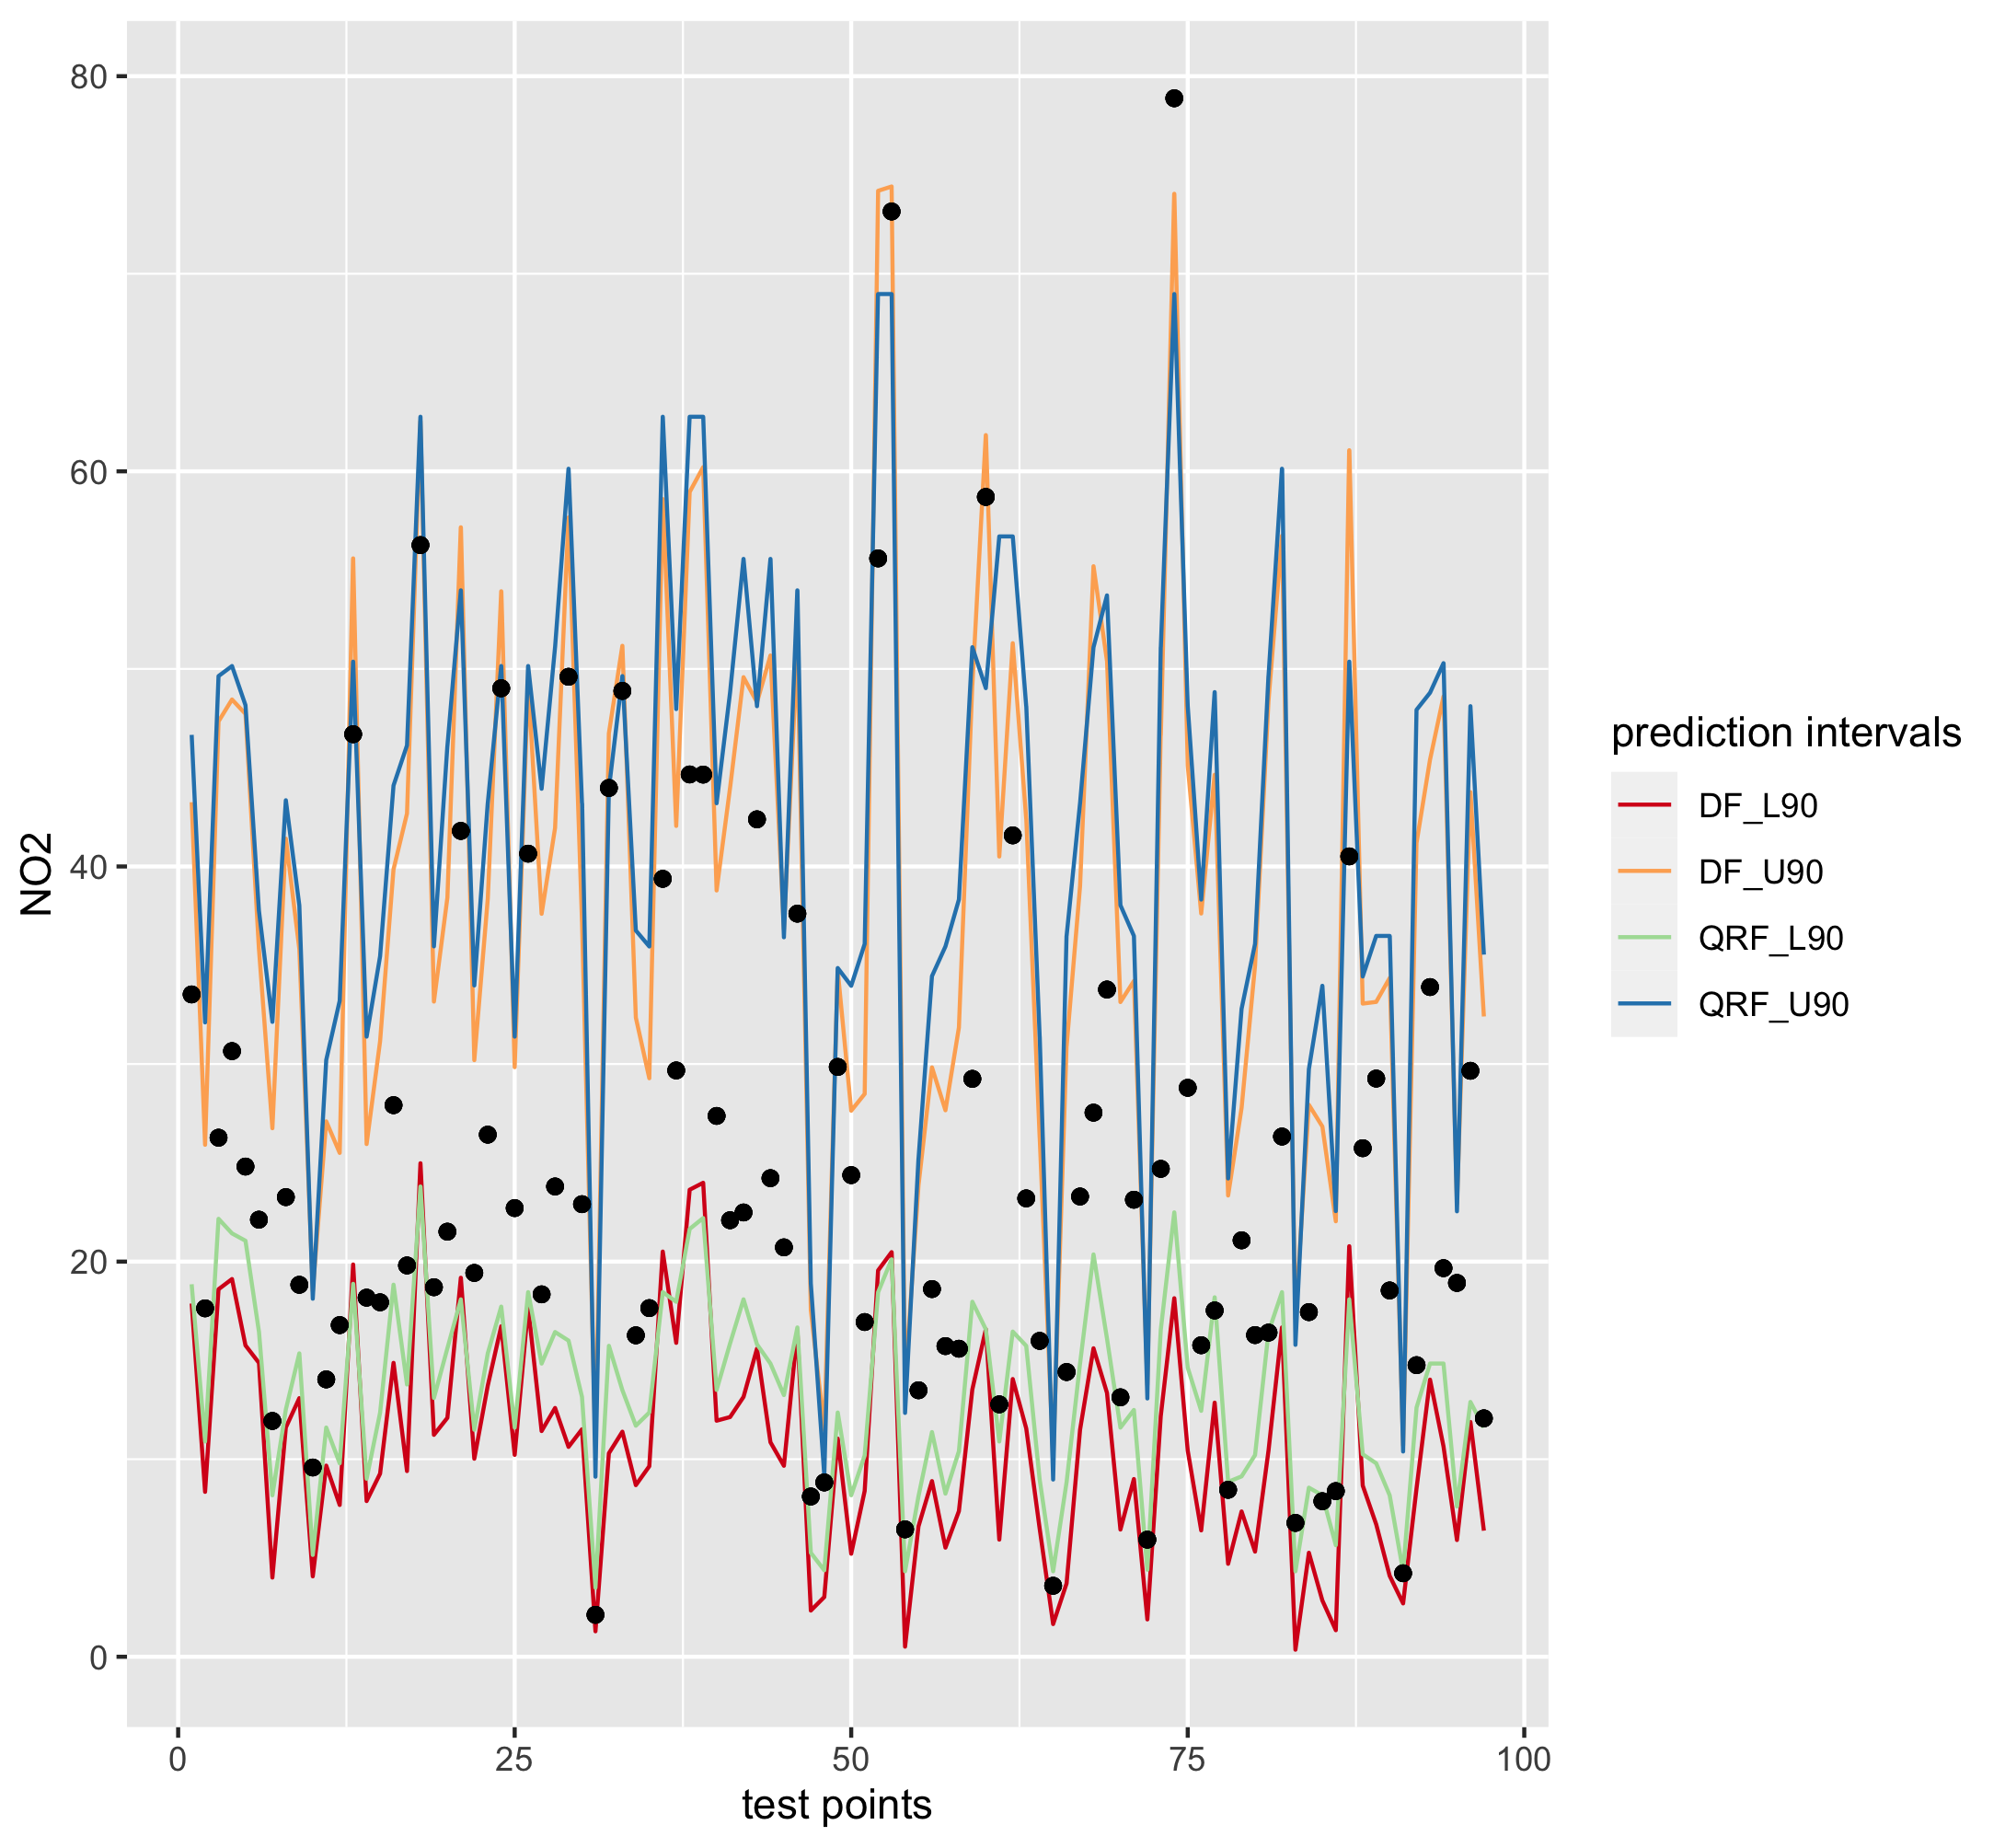
\includegraphics[scale = 0.2]{fig/qrf_df.png}
\caption{The 90\% prediction intervals predicted by DF and QRF. The black dots indicate observations in the test dataset.}
\label{distvsquant}
\end{figure}

\begin{figure}
\centering
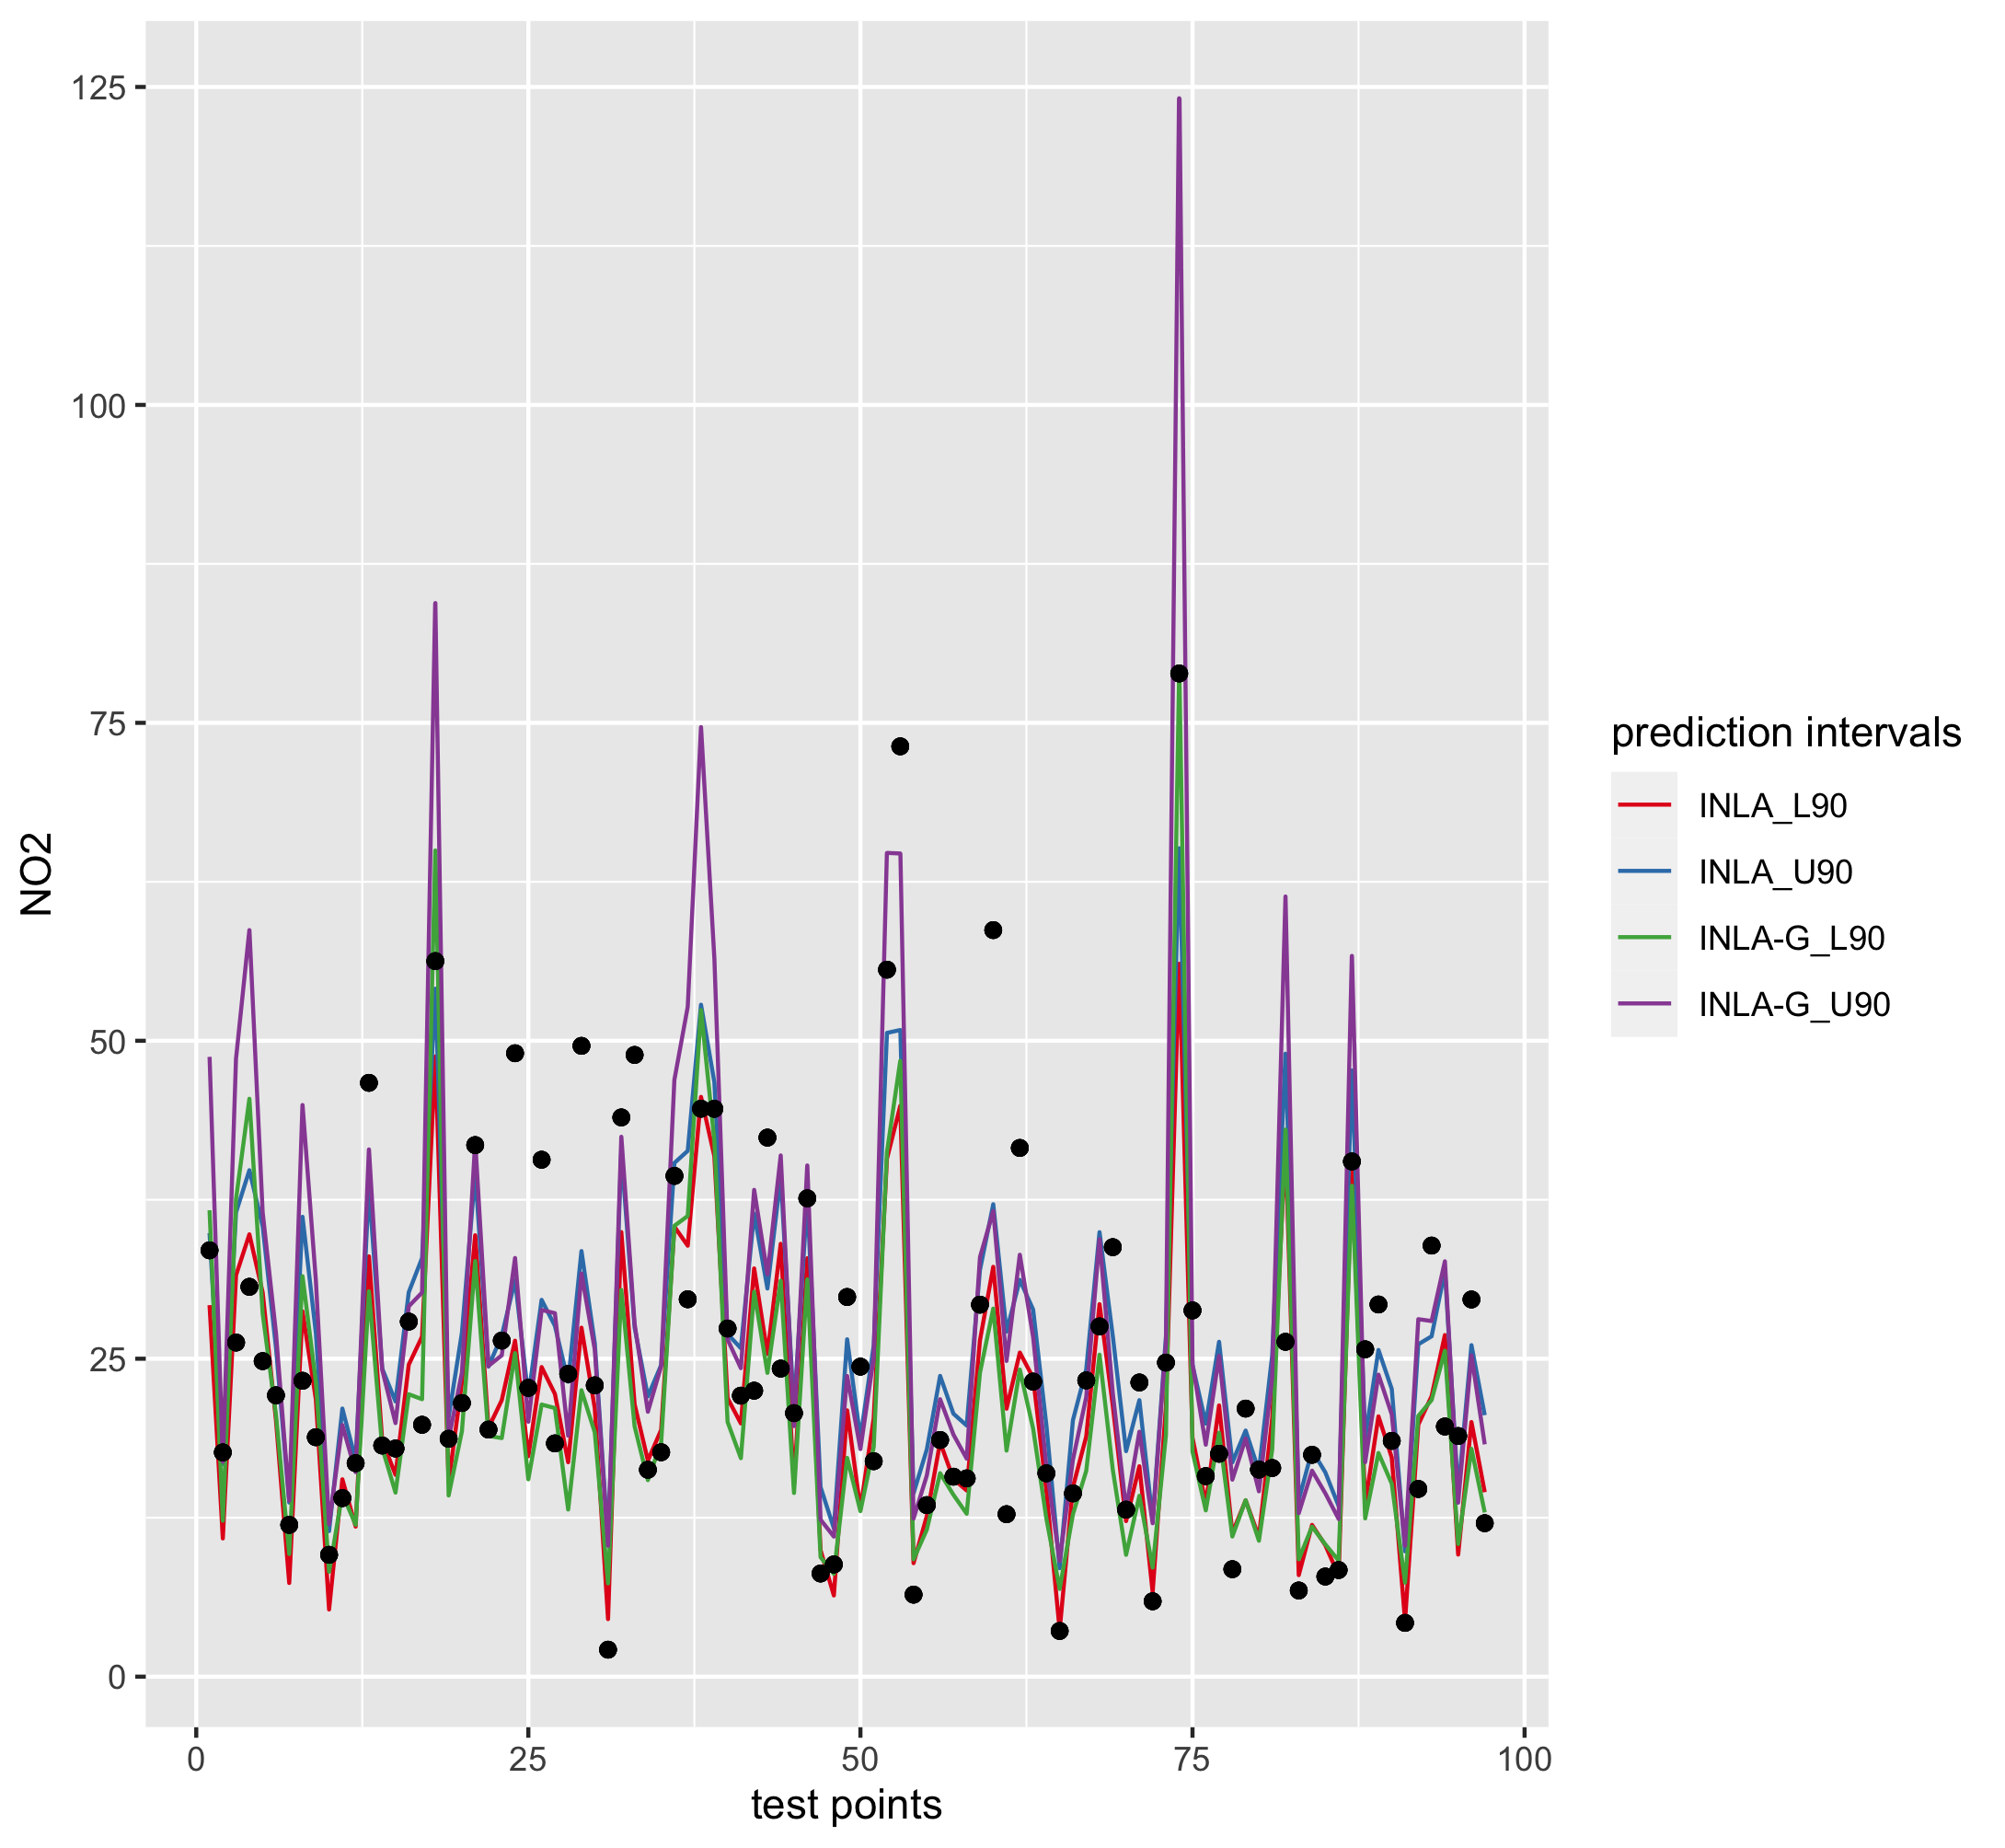
\includegraphics[scale = 0.2]{fig/INLA_pred.png}

\caption{The 90\% prediction intervals predicted by INLA and INLA-G. The black dots indicate observations in the test dataset.}
\label{inlapred}
\end{figure}

\begin{figure}
\centering
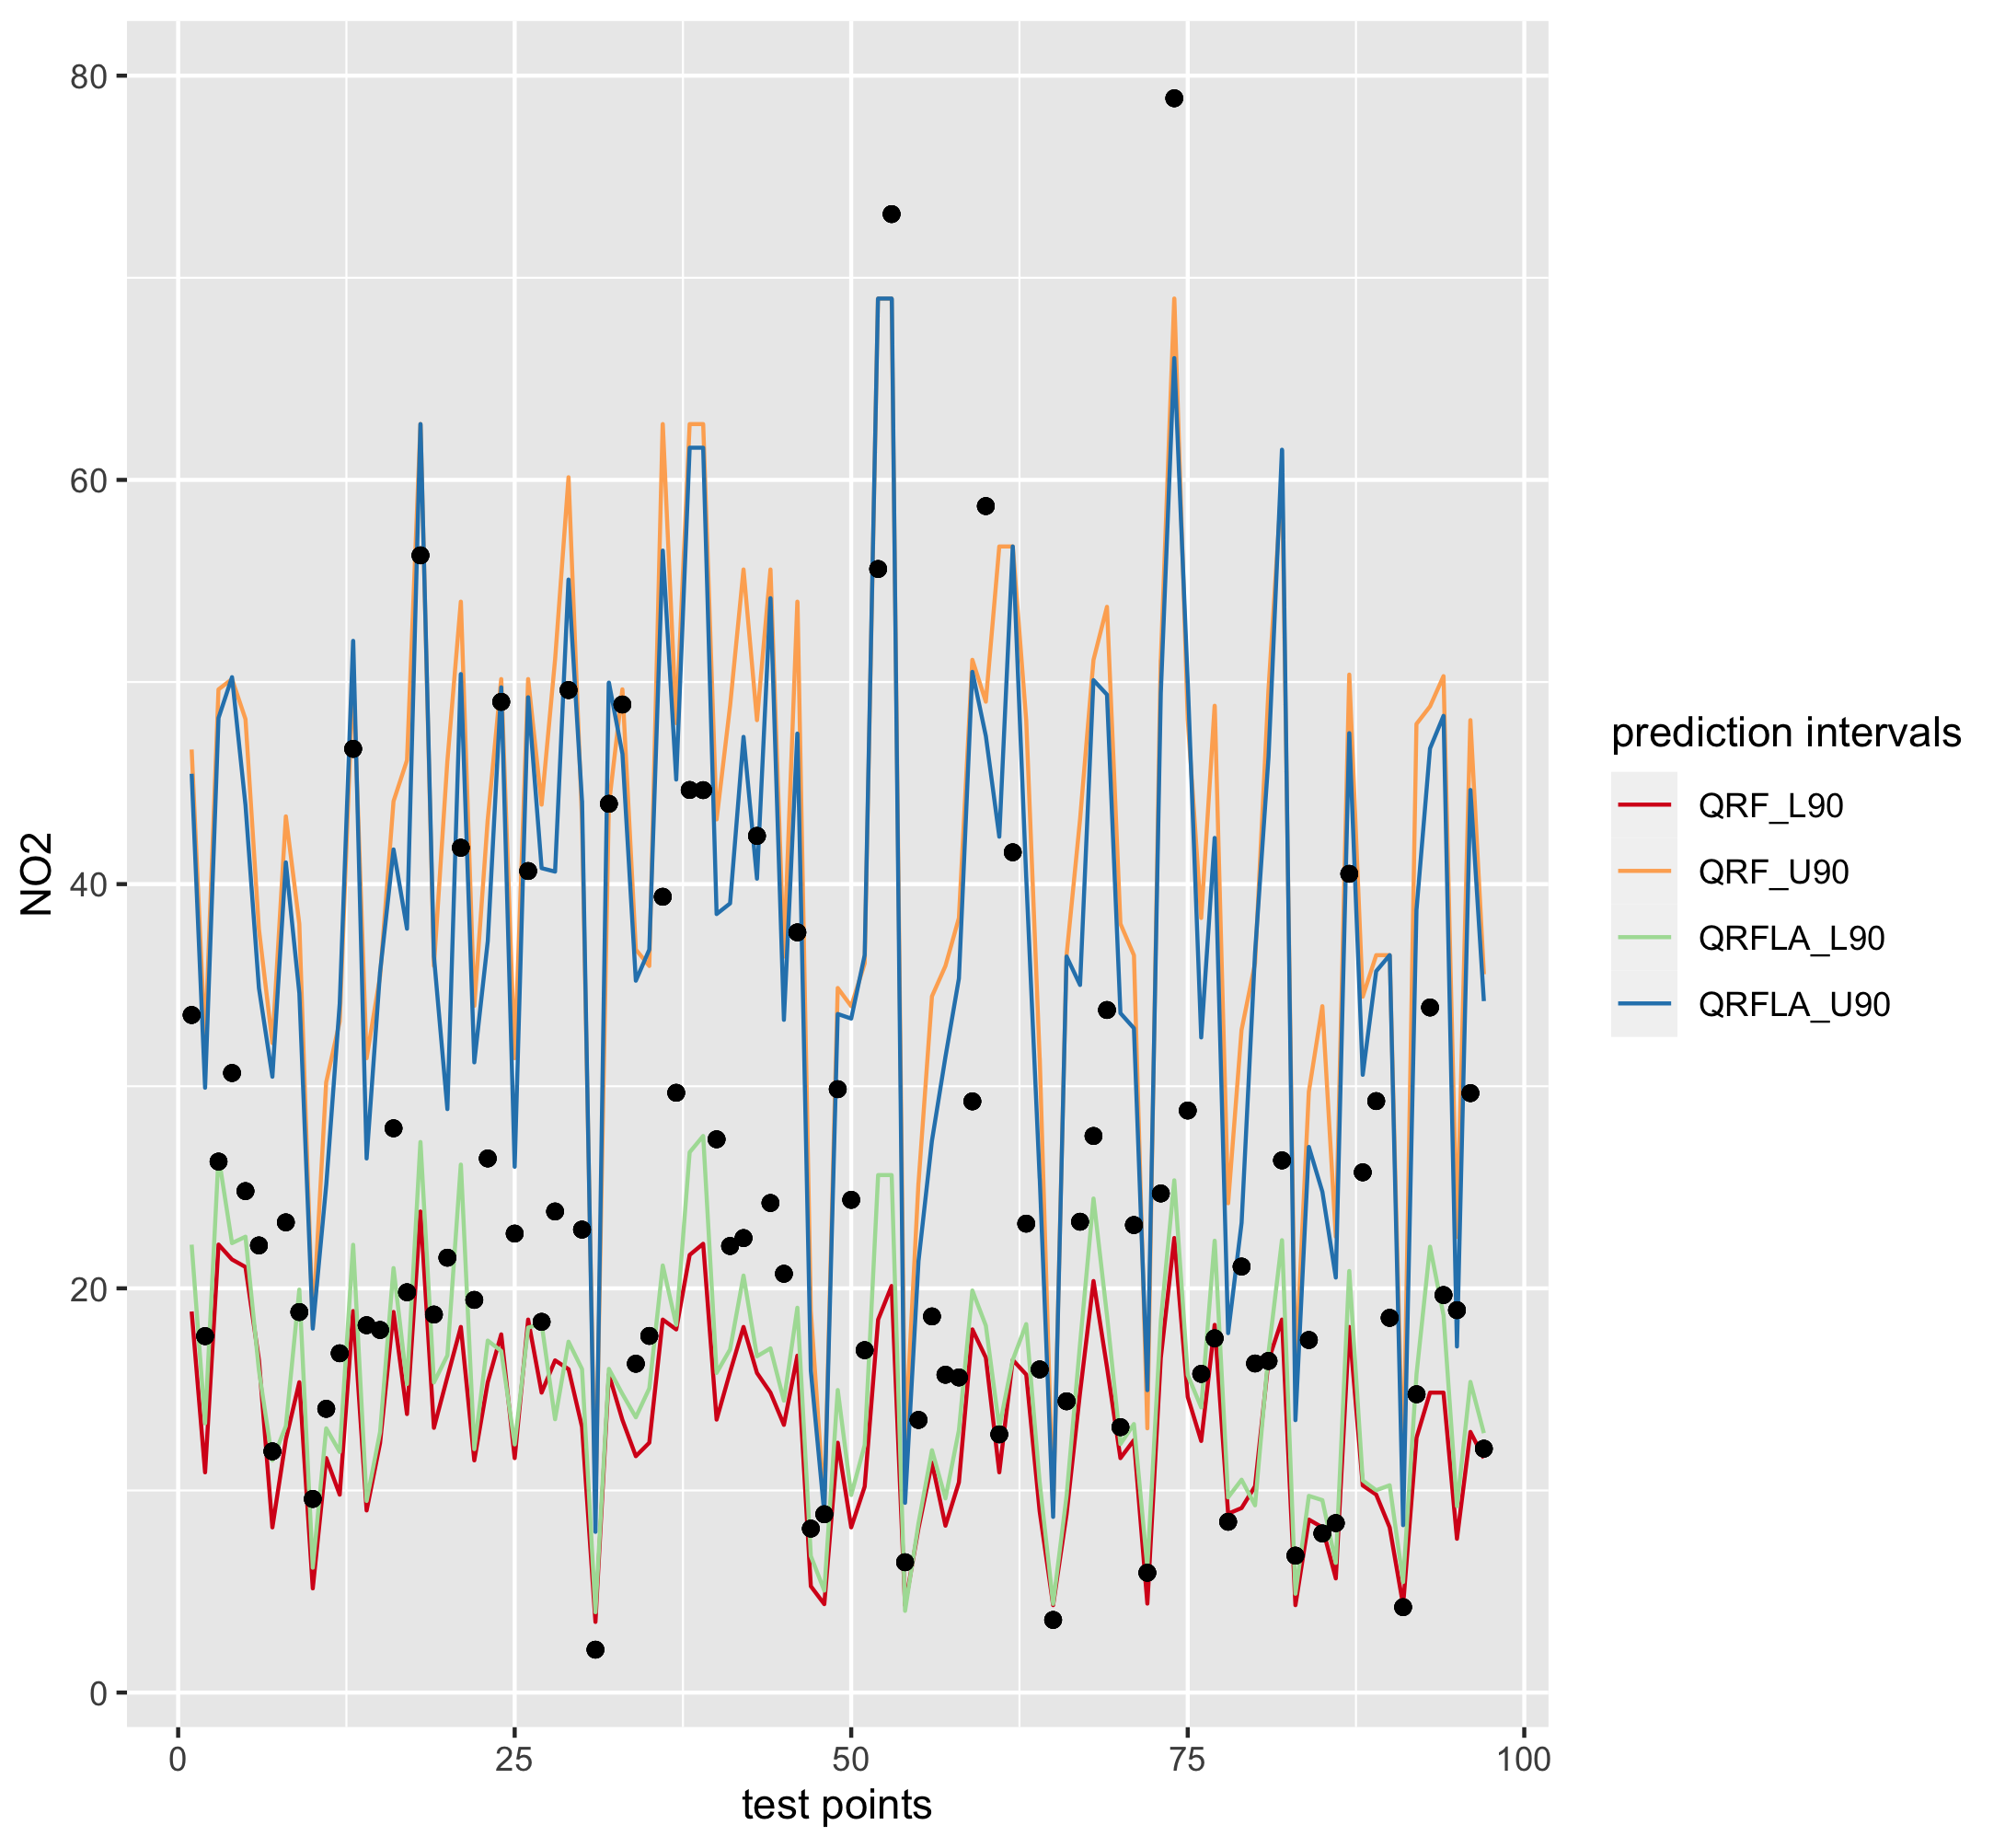
\includegraphics[scale = 0.2]{fig/qrf_qrfla.png}
\caption{The 90\% prediction intervals predicted by QRF and QRFLA. The black dots indicate observations in the test dataset.}
\label{qrrfla}
\end{figure}


\subsection{Model Interpretation} 
%For a linear model the best explanation model is the linear model itself but it is harder to interpret ensembling models \citep{NIPS2017_8a20a862}, which we used SHAP \citep{NIPS2017_8a20a862}.

SHAP values are calculated for RF and XGB methods using all the data. The variables are ranked by their variable importance, which is calculated as the sum of SHAP magnitudes over all the samples. It can be observed from \cref{fig:rfxgbshap} that the variable rankings and the pattern of variable impacts on model output are similar. Both methods ranked road\_class\_2\_100 at the top. The variable importance calculated by the SHAP indicates a pattern that matches well with our expectation in the emission sources (e.g. high pollution close to primary roads). To illustrate, we observe a positive trend of SHAP values along with road\_class\_2\_100 values, this matches with the explanation that areas with higher primary road density generally experience higher NO$_2$ concentrations.

To analyse the effect of each covariate in the INLA model, we firstly normalised all the covariates (by subtracting the mean and dividing the centred columns by their standard deviations) and used all the data to fit the INLA model. road\_class\_2\_100 has the highest effect (mean = 4.37), follows by the population\_3000 (3.08), these are consistent to the XGB variable importance (\cref{fig:rfxgbshap}b ). Then, the road\_class\_3\_300 (3.00) has a notably higher effect (besides the top 2) than other covariates, which has coefficients from 0.72 to 1.88. This differs from the XGB and RF variable importance which ranked the population\_1000 higher above, while in the INLA model the population\_1000 has the lowest effect (0.72). This may be because of the high correlation between population\_1000 and population\_3000, as SHAP is a permutation test, it ignores the dependency between covariates. In general, both geostatistical and ML methods estimated covariate effects match their physical explanations. The statistics (mean, standard deviation, mode) and predicted quantiles of each coefficient are shown in the supplementary material figure 3. 
% do they give the same interpretation?

\begin{figure}
\begin{subfigure}{.5\textwidth}
  \centering
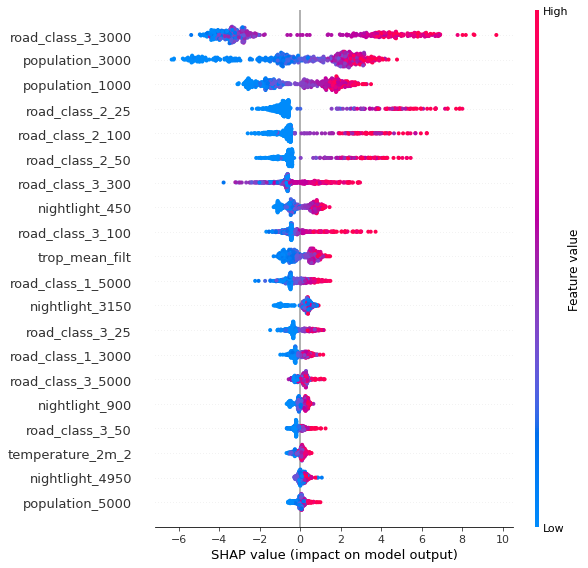
\includegraphics[scale = 0.3]{fig/rfshap.png}
  \caption{}
  \label{fig:sfig1}
\end{subfigure}%
\begin{subfigure}{.5\textwidth}
  \centering
  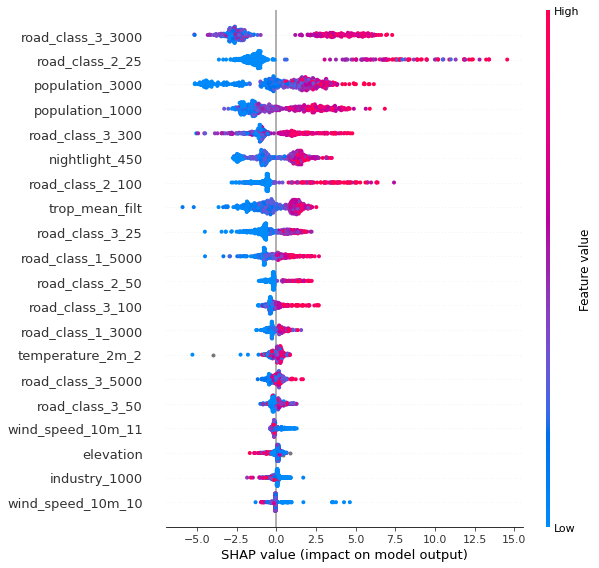
\includegraphics[scale = 0.3]{fig/xgbshap.png}
  \caption{}
  \label{fig:sfig2}
\end{subfigure}
\caption{Variable impact calculated by SHAP (SHapley Additive exPlanations), a) the RF model, b) The XGB model. The covariate ranking is based on the sum of SHAP magnitudes over all the samples. The horizontal axis shows how the effect of a feature changes with the SHAP value of the feature (indicated by the brown to green color bar). The SHAP value is calculated as the conditional mean (conditional to the features that are not used for making the prediction) of the prediction. For example, the low values of the feature “road\_class\_2\_100”, shown in dark brown, correspond mostly with low SHAP values (points to the left). This can be explained that usually the less local road, the less pollution, considering other effects. High values in “road\_class\_2\_100” also contribute greatly to the predictions.
}
\label{fig:rfxgbshap}
\end{figure}
  

The differences between the predicted NO$_2$ and the mean of the spatial random field (\cref{randomfield}) indicates the effects of covariates. The highest values of the mean of the spatial random field are shown in the south-west (48.7758° N, 9.1829° E, in and around the German city Stuttgart). Relatively high values can be observed in northern, southern and western Germany. Compared to \cref{INLApred}, the areas close to the Stuttgart (Germany) region where the mean values of the spatial random field are high corresponds to the high magnitudes of NO$_2$ concentrations. Also, the differences between the observations and predictions are relatively large in magnitudes in this region. To facilitate visualisation, we also calculated the differences between INLA model predictions and the observations  (supplementary material, figure 2).  

 
  

\begin{figure}
\centering
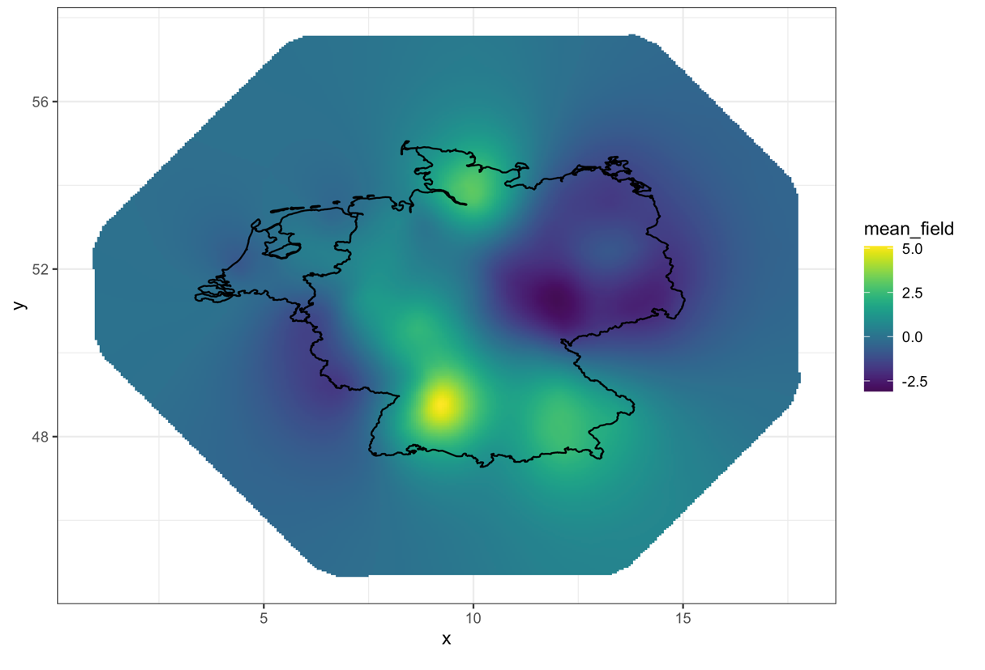
\includegraphics[scale = 0.5]{fig/mean_randomfield.png}
\caption{Mean of the spatial random field fitted by the INLA model. The polygons indicate Dutch and German boundaries.}
\label{randomfield}
\end{figure}


\begin{figure}
\centering
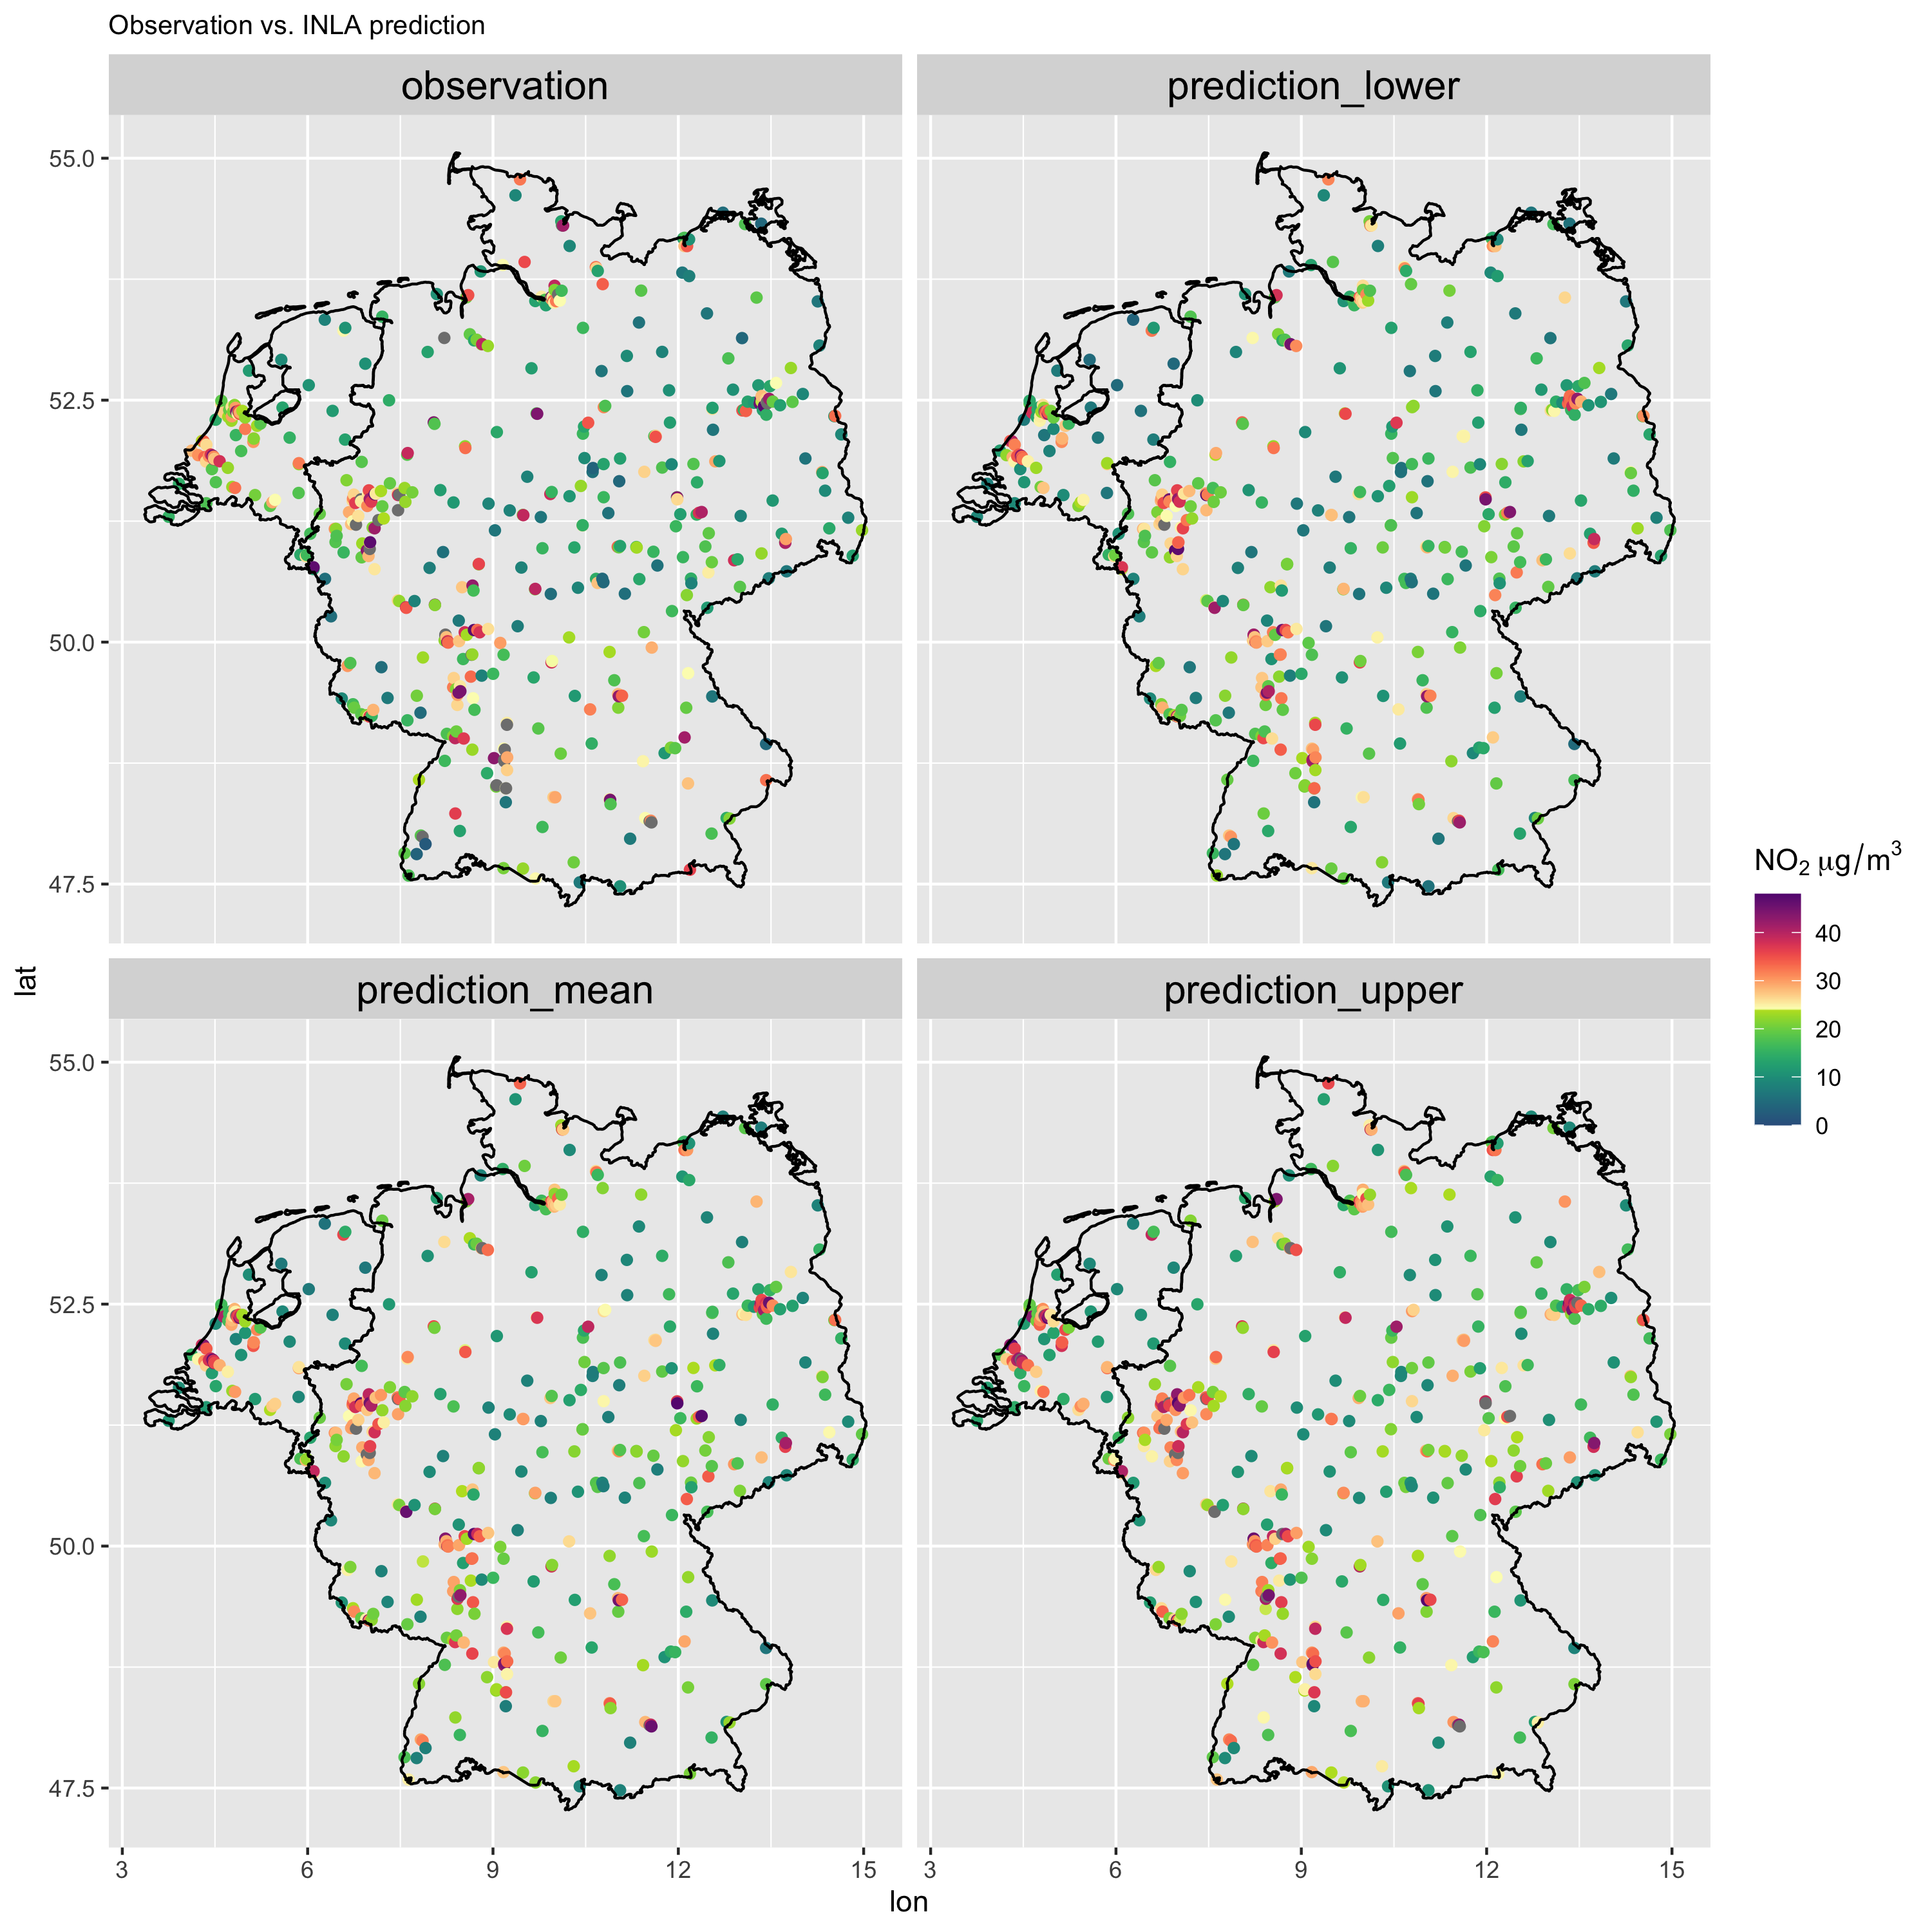
\includegraphics[scale =0.1]{fig/pred_11var.png}
\caption{INLA predicted NO$_2$ at the ground stations with mean (prediction\_mean), high (prediction\_high, 0.975) and low (prediction\_low, 0.925) quantiles and the observed NO$_2$ (observation). The polygons indicate Dutch and German boundaries.}
\label{INLApred}
\end{figure}

%\begin{figure}
%\centering
%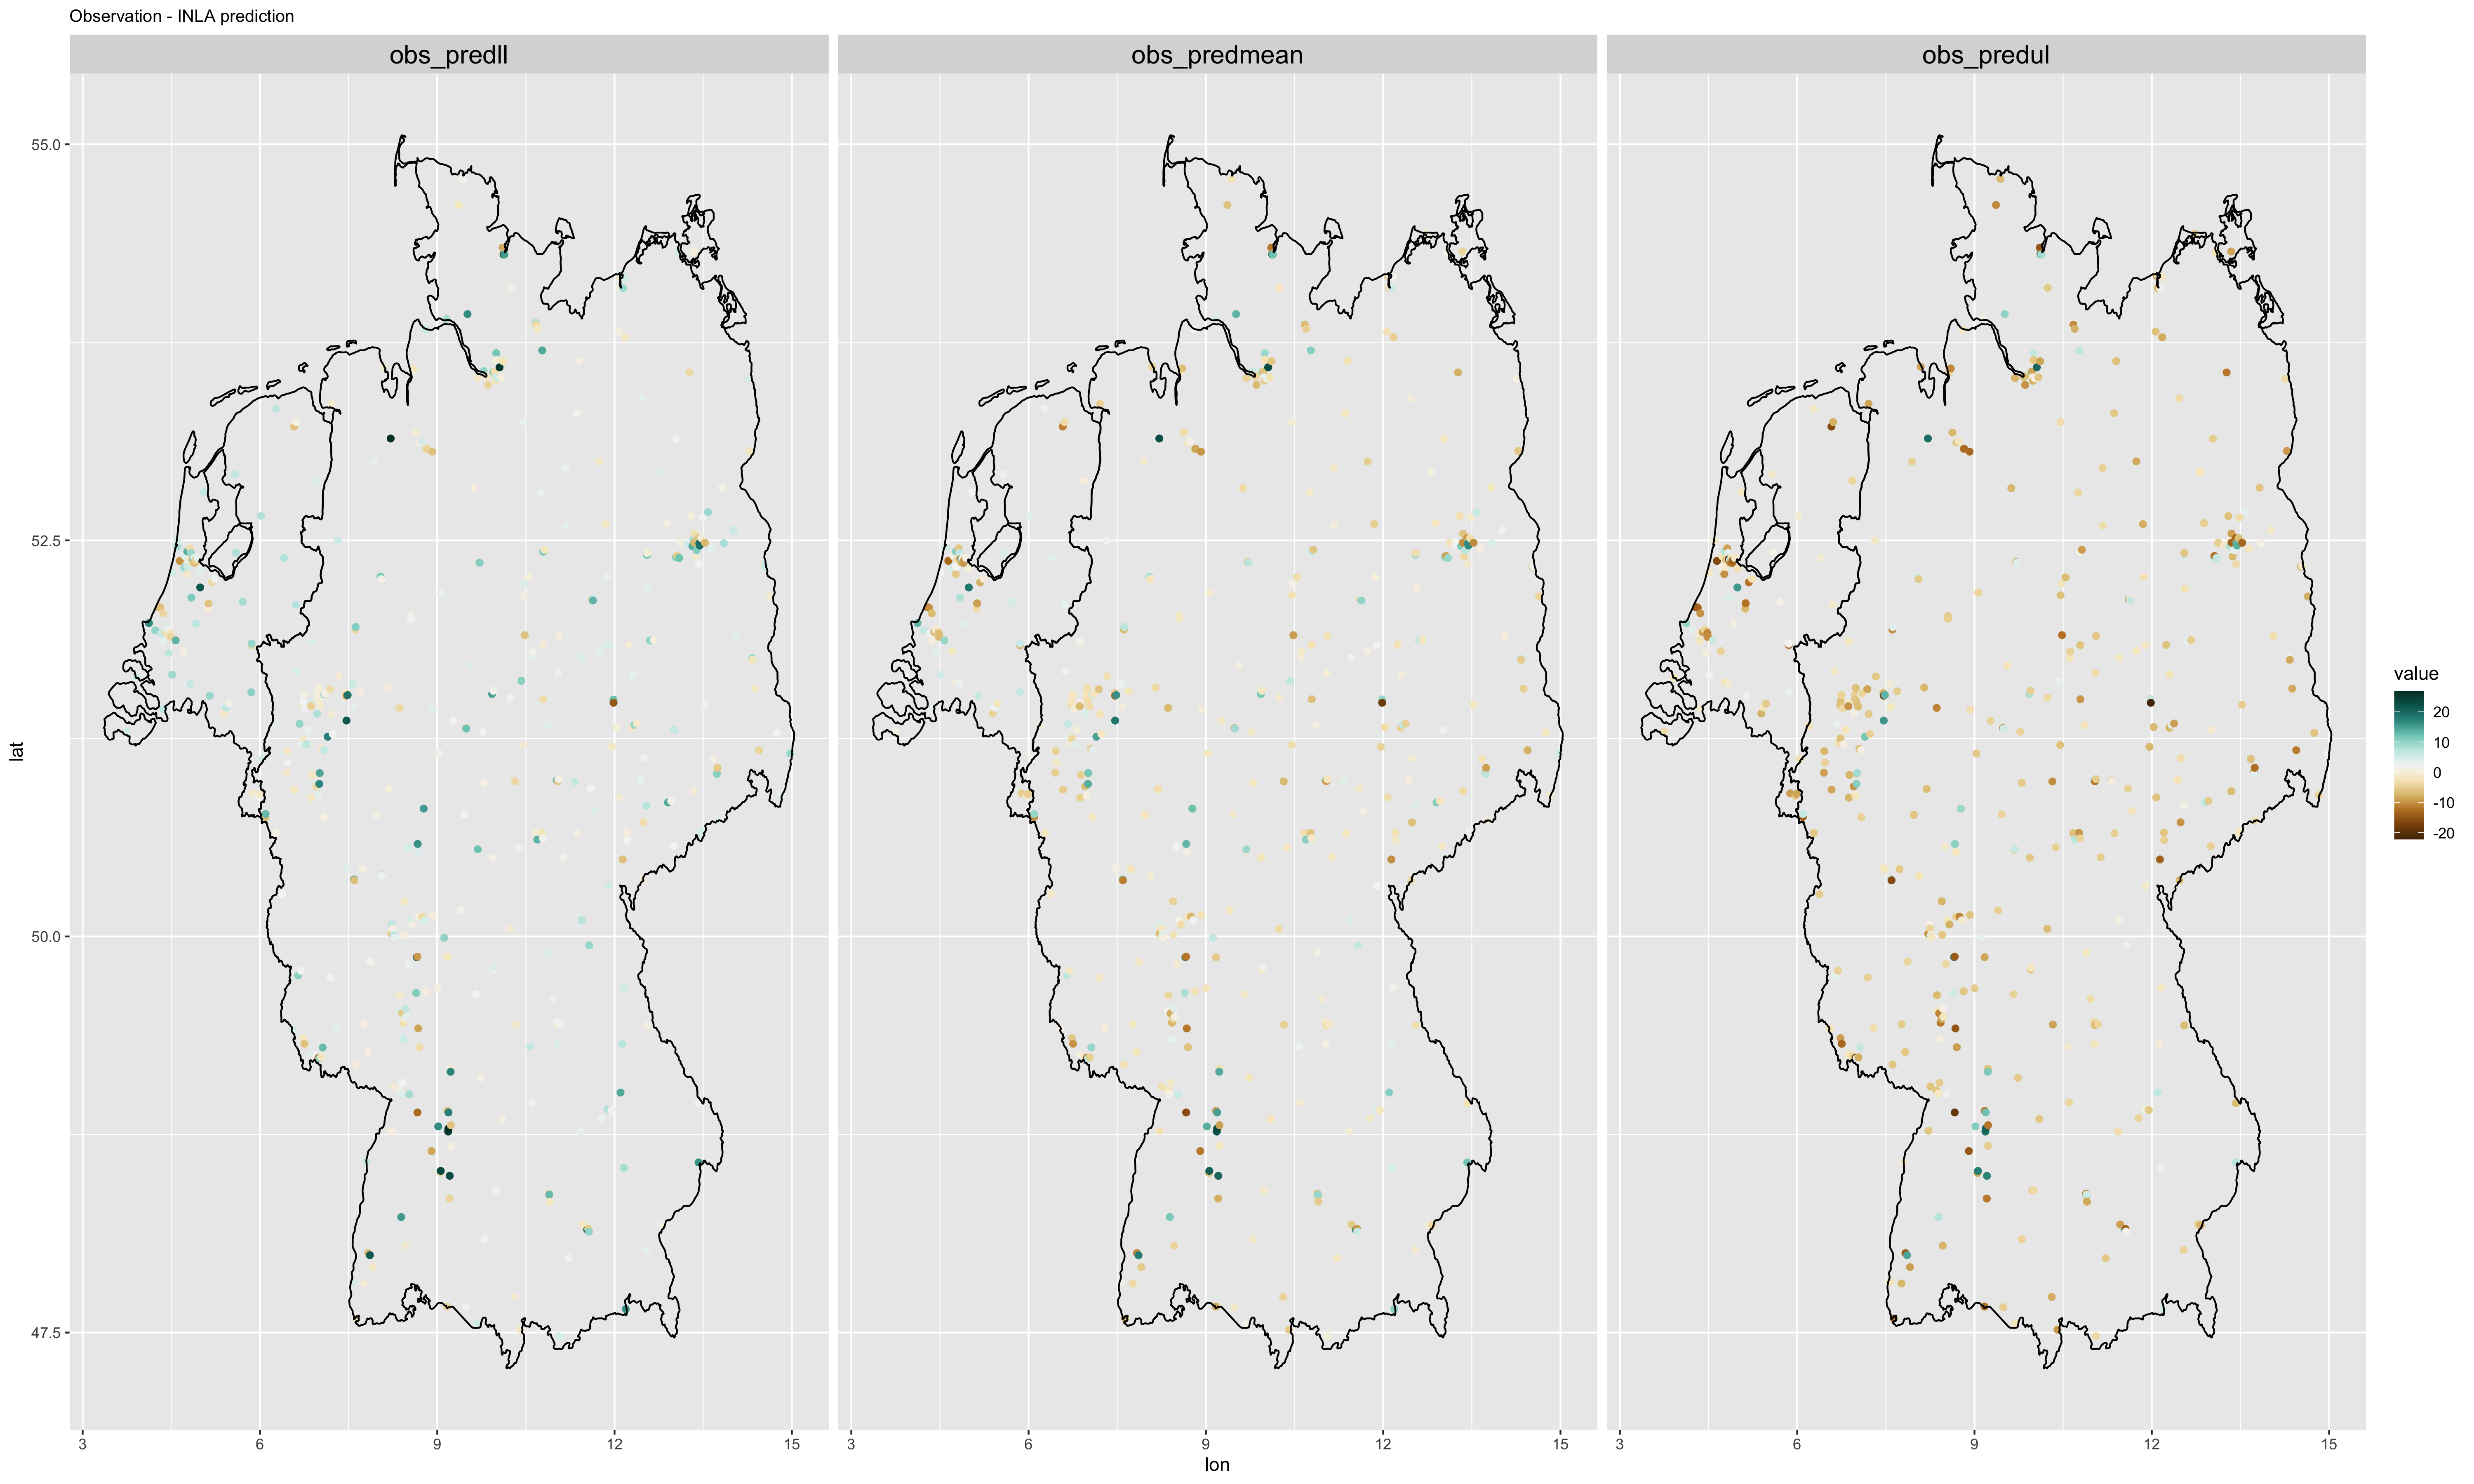
\includegraphics[scale = 0.05]{fig/dif_obs_INLA_11var.png}
%\caption{Differences between INLA predicted NO$_2$ at mean, high (0.975) and low (0.925) quantiles and the observed NO$_2$. The differences (dif) is calculated as substracting predictions (pred) from the observations (obs), i.e. $dif = obs - pred$.}
%\label{difINLA}
%\end{figure}

\section{Discussion}
In this study, we compared spatial and non-spatial models for spatial NO$_2$ prediction in Germany and the Netherlands. The comparison consists of the predicted mean, prediction intervals, and model interpretation. Spatial and non-spatial CV strategies are used to reveal prediction accuracy in different aspects. We also implemented the Lasso post-processed RF and spatial stacked learning for NO$_2$ mapping (which to our knowledge have not been applied in air pollution mapping before) and these two methods considerably improve from the original RF and stacked learning models, respectively. %We propose the same model evaluation strategies to be incorporated in all the model comparison studies. 

Several venues were attempted to further improve the spatial model fitted with INLA. Firstly, as we observed in general worse results at the geographical boundaries (\cref{fig:r2,fig:crps}), we inspected if different meshes with edge-effects fully accounted (e.g. the mesh is sufficiently large for observations at the edge) could improve the prediction accuracy. It turned out that the same performance is obtained. Secondly, we suspected that deviating from the assumed Gaussian distribution causes narrow prediction intervals of the INLA model. However, assuming a Gamma likelihood did not improve the model performance in terms of the accuracy matrix, CRPS and coverage probability. We also experienced the square transformation of the observations and the use of the log-normal likelihood but that also decreases the model performance. Thirdly, we additionally added two factor variables, namely ``country code \footnote{DE for Germany and NL for the Netherlands} and ``urban types" \footnote{rural, urban, city centre according to \citep{urbantype}}. However, that also does not increase the model performance. In future works, using a different spatial model (e.g. by specifying different hyperparameters), using the country and urban types as mixed-effects, and modelling spatial varying coefficients may improve the modelling results. Major improvement may also be achieved by integrating mobile sensing measurements and other geospatial predictors (e.g. traffic count, urban morphological matrix) \citep{moragaetal17}.

%If the prediction interval can be calculated, we can also visualise the uncertainty with the length of a certain quantile of prediction intervals \citep{shaddick2015spatio}.   
 

In our study, we designed our spatial-blocked CV to disaggregate the model accuracy metrics from global to spatial-block-wise error. This method has the benefit that we know exactly which data is used for training and which for testing, however, as \cite{wadoux2021spatial} pointed out, this type of method may experience the extrapolation problem. We reduce this problem by selecting a relatively small block size. Specifically, we chose the 2-degree cell size as with it we have a relatively balanced number of stations and stations of different urban types and can better visualise the geographical pattern. With a smaller cell size, the information in each grid cell is closer to a single or a small combination of ground stations and gives less information about the areas surrounding each ground station. Applying the typical random k-fold or leave-one-out-cross-validation and then calculating the accuracy in each block could avoid the extrapolation problem. In the supplementary material figure 6, we show the NSE of the XGB in each spatial block after applying the random 10-fold CV and compared it with the spatial-blocked CV. 
 
 %We experimented with smaller cell sizes such as 1 degree, which leads to 64 grid cells.  

%\cite{wadoux2021spatial} argues that there is a conflict between achieving spatial independence between test and training data, and avoiding extrapolation in CV for environmental mapping. 
There has been a debate in how to faithfully assess the model accuracy with spatially correlated data. Several studies believe the typical k-fold CV causes overly optimistic accuracy assessment and developed "spatial CV" methods  \citep{brenning2012spatial,meyer2018improving} and they have been advocated in environmental mapping \citep{ploton2020spatial}. However, the spatial CV does not seem to solve the overly optimistic accuracy assessment problem as the problem is caused by insufficient samples in the feature space. The spatial CV causes extra extrapolation problem \citep{wadoux2021spatial} without solving the real problem.  

 
%Several methods have been developed to reduce the spatial dependency between training and test data for spatial prediction. The methods are commonly referred to spatial CV \citep{brenning2012spatial,meyer2018improving} and they have been advocated in environmental mapping \citep{ploton2020spatial}. For example, \cite{ploton2020spatial} criticised the overly optimistic accuracy obtained in environmental mapping without using spatial CV. However, on one hand, it is obvious that that spatial CV causes the extrapolation problem \citep{wadoux2021spatial}. %\cite{wadoux2021spatial} proposed to encourage the design-based approach, but in practice it is not always possible due to data availability. On the other hand, it is unclear the necessity of achieving the spatial independence between training and test data. CV is the most effective when the distributions of the feature values of the test data spread over that of the training data, and what we try to avoid is that the feature values of the test data clustered at a part of the feature values of the training data. This means we should look into the feature space to evaluate how effective the CV is. Dividing data into spatial blocks seems not directly relevant to a solution. 

A sensible accuracy assessment approach is to look into the differences between the distribution of the feature values  of the population and the samples. A progress is made by \cite{meyer2021predicting}, who proposes the area of applicability, which quantifies the differences between feature values used in training and for prediction and used the magnitude of it as an indicator for applicability. The method adds a useful diagnostic tool for applying machine learning models to spatial prediction. However, as is discussed in \cite{meyer2021predicting}, there are several limitations. One important limitation is that there is no quantitative associations between \textit{how "applicable" an area is} and \textit{the prediction errors or uncertainty}. %In another word, it is not quantifiable how much the error would increase if extrapolating occurs. %Another problem is that the method simply aggregates the distance in the feature space, which may not match with how the joint effects of covariates are considered in a machine learning or statistical model.  



The model performance differs greatly between the three road and population situations. The ``far" situation obtained the best modelling accuracy while the ``tr-hp" the worst. This is likely due to the fact that the urban NO$_2$ process is more complex due to urban forms and traffic conditions. This may also indicate that more detailed traffic counts and meteorological data are needed for modelling the NO$_2$ emission sources.  

Different from non-parametric models such as ensemble trees, a parametric  spatial model fitted with INLA as the one developed in our study requires feature selection and the assumption of the distribution of the response. Several studies used the whole dataset for variable selection and then use selected variables for CV \citep{lu2020land,larkin2017global}. This may however lead to an information leak as the validation data is also used in CV. To avoid this problem, one can include the variable selection process in each CV, i.e. use the same training data for variable selection and test. However, variable selection in each run could introduce additional error and uncertainty, therefore, a determined set of covariates may be preferred. We obtain a fixed set of selected variables while reducing information leakage to a negligible level by choosing only the variables that are selected 90\% -100\% times of all the bootstraps of Lasso.

Using the geostatistical method to stack learners obtained higher prediction accuracy in terms of the mean prediction compared to the non-spatial stacking. This suggests the complex response-covariate relationships modelled by the ML learners do not fully capture the spatial process. The  spatial stacked models obtained the highest prediction accuracy and with high-performance computation, it is possible to apply them to a large-scale and at a high resolution. The limitation of such stacked methods is that they cannot be used to analyse the effects of covariates and therefore NO$_2$ emission sources. But these models could be a reference to the level of accuracy a statistical predictive model could reach with the data available and the base learners.% are local or global models.

As ground stations of NO$_2$ are predominately close to traffic, the predictions might be biased towards higher NO$_2$ concentrations. This problem is referred to preferential sampling, which occurs when the sampling design process is dependent on the spatial process. A few methods have been developed to address this problem, using Monte Carlo estimates for the likelihood function \citep{diggle2010geostatistical} or numerical methods \citep{dinsdale2019methods}. %For example,  higher sampling probability can be given to rural areas than in traffic regions. However, excluding stations closer to traffic for a more balanced sampling design may make it more difficult to capture the more complex and hazardous NO$_2$ process near traffic.
A much less technical approach to reduce the bias might be to include sufficient traffic-related covariates and a model capable of capturing the traffic-NO$_2$ relationships. In this sense, NO$_2$ mapping may experience a promising improvement when more traffic counts and emission data become available in future.  

An advantage of the spatial model is that it could quantify the uncertainty of the spatial covariance matrix in terms of the hyperparameters of the covariance function, as well as block averages or block totals, at any aggregation level. Examples are block or point-to-area Kriging. In practice, the block averages are often more of interest than values at points, and we commonly would like to aggregate data at different spatial and spatiotemporal levels. For example, with mobile sensor measurements. Even though we could derive a prediction interval from the non-spatial method, the prediction interval is derived at the point level. At a block level, the uncertainty can only be formally quantified while accounting for the spatial dependency between points within a block. This is a distinction between non-spatial and spatial models, for example, blocked Kriging, whose Kriging variance is very sensitive to the behaviour of the variogram at within-block distances. 

\section{Conclusion}
We proposed a model comparison process to comprehensively compare between models considering not only the predicted mean but also prediction intervals and model interpretation. We also showed that the information provided by commonly single-used non-spatial CV may miss reflecting model behaviours. With the model comparison process, we compared the use of spatial models and ML models for the spatial prediction of NO$_2$ in Germany and the Netherlands and found noticeable differences in their limitations and strength. The  spatial models are preferred especially for urban area prediction and provide the spatial process of observations and indicate the insufficient modelling of spatial random-effects of fixed-effects. But the uncertainty assessment of spatial models, which is commonly known as a strength, fails to provide a prediction interval that meets the expectation. The QRF and DF obtained satisfying prediction intervals, with the DF slightly more capable of predicting the extremes. Using Lasso to postprocess random forest increases model performance and reduces model variance. Using a spatial model to stack learners obtained the highest accuracy in terms of the mean prediction. Despite the NO$_2$ observations follow closer to a Gamma distribution than a Gaussian, the use of a Gamma likelihood in the spatial model and Gamma objective in the XGBoost obtained much worse results than using a Gaussian likelihood or objective. By comparing with the non-spatial stacked ensemble learning, spatial stacked ensemble learning suggests the necessity of modelling the spatial process.  
%We propose the same model ev

\newpage
\bibliographystyle{abbrvnat}

\bibliography{references}
\end{document}

Other: the newest boosting technique, Catboost, gives the best cross validation results, with same learning rate as xgboost and number of iterations. But it's not convenient for now to ensemble it as it is not yet in h2o. 

                    Catboost
RMSE          7.0 
RRMSE         0.3 
IQR           6.4 
rIQR          0.3 
MAE           5.0 
rMAE          0.2 
rsq           0.70 
explained\_var 0.70

with spatial cv
                    INLA 
                    
RMSE          10.0900074
RRMSE          0.3023047
IQR           11.6697717
rIQR           0.3894527
MAE            7.4846970
rMAE           0.2242679
rsq            0.3630397
explained\_var  0.4319317
 
 Lasso
RMSE	10.0900074			
RRMSE	0.3023047			
IQR	11.6697717			
rIQR	0.3894527			
MAE	7.4846970			
rMAE	0.2242679			
rsq	0.3630397			
explained\_var	0.4319317	

RF
RMSE	9.6393525			
RRMSE	0.2888581			
IQR	11.6795936			
rIQR	0.3899266			
MAE	7.2699949			
rMAE	0.2178434			
rsq	0.4176984			
explained\_var	0.4752084			
covprob90	0.9063574	

XGB 
RMSE	9.6618743			
RRMSE	0.2895155			
IQR	10.1181299			
rIQR	0.3379141			
MAE	7.0342845			
rMAE	0.2107836			
rsq	0.4140045			
explained\_var	0.4960338

Stacked INLA
RMSE           8.48140767
RRMSE          0.25475534
IQR           10.50499614
rIQR           0.35099809
MAE            6.53715007
rMAE           0.19644237
rsq            0.54917218
explained\_var  0.55811686
cor            0.75390795
covpr95      0.21804124
covprob90      0.17989691
covprob50      0.08092784


If I choose clustered points with high prob (big city?), the result is similar to random sampling, and better accuracy. 

 

If I choose scattered points with high prob (does it mean more rural points?), there is very little randomness. result is also worse. --> the reason for scattered points with high prob. is because they contain more info?
there are a lot more clustered points (as the hist. peak at small prob). so the scattered points will be selected first, that is the reason there is little randomness. 

 
\subsection{Variable importance}
   \begin{table}[!htbp] \centering 
    \caption{Variable importance ranked by XGBoost and random forest. The ranking is based on variable importance averaged over 20 times bootstrapping.} 
    \label{vimp} 
  \begin{tabular}{@{\extracolsep{5pt}} ccc} 
  \\[-1.8ex]\hline 
  \hline \\[-1.8ex] 
  rank & XGBoost & Random Rorest \\ 
  \hline \\[-1.8ex] 
  1 & population\_3000 & population\_3000 \\ 
  2 & road\_class\_3\_3000 & road\_class\_2\_100 \\ 
  3 & population\_1000 & road\_class\_3\_3000 \\ 
  4 & nightlight\_450 & population\_1000 \\ 
  5 & road\_class\_2\_100 & nightlight\_450 \\ 
  6 & road\_class\_3\_300 & nightlight\_3150 \\ 
  7 & road\_class\_1\_5000 & population\_5000 \\ 
  8 & nightlight\_3150 & road\_class\_3\_300 \\ 
  9 & road\_class\_3\_100 & nightlight\_900 \\ 
  10 & population\_5000 & road\_class\_3\_5000 \\ 
  11 & trop\_mean\_filt & road\_class\_2\_300 \\ 
  12 & radiation & road\_class\_3\_100 \\ 
  13 & nightlight\_900 & nightlight\_4950 \\ 
  14 & road\_class\_3\_5000 & trop\_mean\_filt \\ 
  15 & road\_class\_1\_100 & road\_class\_1\_5000 \\ 
  16 & nightlight\_4950 & industry\_5000 \\ 
  17 & temperature\_2m\_2 & road\_class\_1\_3000 \\ 
  18 & road\_class\_1\_3000 & temperature\_2m\_2 \\ 
  19 & elevation & road\_class\_2\_500 \\ 
  20 & industry\_5000 & elevation \\ 
 
  \hline \\[-1.8ex] 
  \end{tabular} 
  \end{table} 
  
  
  \begin{table}[!htbp] \centering 
  \caption{} 
  \label{} 
\begin{tabular}{@{\extracolsep{5pt}} ccccc} 
\\[-1.8ex]\hline 
\hline \\[-1.8ex] 
 & LA & RF & XGB & RFLA \\ 
\hline \\[-1.8ex] 
RMSE & $7.54$ & $7.40$ & $7.10$ & $7.24$ \\ 
RRMSE & $0.32$ & $0.32$ & $0.30$ & $0.31$ \\ 
IQR & $8.42$ & $7.22$ & $6.27$ & $7.26$ \\ 
rIQR & $0.39$ & $0.34$ & $0.29$ & $0.34$ \\ 
MAE & $5.67$ & $5.41$ & $4.98$ & $5.26$ \\ 
rMAE & $0.24$ & $0.23$ & $0.21$ & $0.23$ \\ 
rsq & $0.66$ & $0.67$ & $0.70$ & $0.68$ \\ 
explained\_var & $0.66$ & $0.67$ & $0.70$ & $0.68$ \\ 
\hline \\[-1.8ex] 
\end{tabular} 
\end{table} 

\begin{table}[!htbp] \centering 
  \caption{Cross-validation results of 20 times boot-strapping.} 
  \label{cv} 
\begin{tabular}{@{\extracolsep{5pt}} ccccccc} 
\\[-1.8ex]\hline 
\hline \\[-1.8ex] 
   &LA & RF& XGB & stacked & INLA& stacked INLA  \\ 
\hline \\[-1.8ex] 	
 
RMSE & $7.8$ & $7.5$ & $7.4$ & 7.2 & 7.5&7.1\\
%RRMSE & $0.3$ & $0.3$ & $0.3$&  &0.3\\
IQR & $8.5$ & $7.5$ & $6.9$  &  &7.2\\ % for non-gaussian error this makes little sense
%rIQR & $0.4$ & $0.3$ & $0.3$ & &0.3\\
MAE & $5.9$ & $5.5$ & $5.3$  & 5.2 & 5.5&5.3\\
%rMAE & $0.2$ & $0.2$ & $0.2$ &  &0.2\\
NSE & $0.63$ & $0.66$ & $0.67$&  0.68 &0.66 &0.69\\
%explained\_var & $0.63$ & $0.66$ & $0.67$ &&  0.66 &0.69 \\ 
\hline \\[-1.8ex] 
\end{tabular} 
\end{table} 


%Feb 9, 2021 1:55 PM j.cavieres.g:  If you are talking about the comparison between models (ML, spatial linear models, hierarchical models, etc) based on the distribution of the observed data, I have never seen this. What is my opinion? I think that ML models are more interested in the prediction than in the inference. If they generalize well the prediction of a particular phenomenon then that model is 'good'. In our case it is very interesting to see that the machine learning model using a Gamma distribution has poor statistical performance compared with INLA, but probably that model can predict better. For the above is necessary to do an analysis where we can evaluate if that model is overfitting or not. 




\begin{abstract} 
NO$_2$ is a traffic-related air pollutant that is strongly associated with cardiovascular and respiratory diseases. Ground NO$_2$ monitoring stations measure NO$_2$ concentrations at certain locations and statistical predictive methods have been developed to predict NO$_2$ as a continuous surface to inform decision-making. Among them, ensemble tree-based machine learning methods have shown to be powerful in capturing non-linear relationships between NO$_2$ measurements and geospatial predictors, but it is unclear if the spatial structure of NO$_2$ is also captured in the response-covariates relationships. In addition, most model comparison studies only compare accuracy in the prediction mean at ground stations, but do not consider prediction intervals and model interpretation and the effects of different model evaluation methods. In this study, we dive into the comparison between spatial and non-spatial data models accounting for the above-mentioned aspects. 
Moreover, we implemented a spatial and a non-spatial methods that have not been applied to air pollution mapping before and evaluated stack learning methods with and without modelling the spatial process. We implemented our study using national ground station measurements of NO$_2$ in Germany and Netherlands of the year 2017.
Our results indicate heterogeneous levels of importance of modelling the spatial process in different areas. 
The prediction intervals predicted with ensemble tree-based methods are more satisfactory than with the geostatistical methods. The two new methods implemented each obtained better prediction accuracy compared to the original ensemble tree-based and stacking methods. The probabilistic distribution of the spatial random field estimated by the geostatistical methods could provide useful information for analysing emission sources and the spatial process of observations.  

%, predicting NO$_2$ to 100 m resolution grid. 
%Three cross-validation methods considering different aspects of spatial information are designed to assess the prediction accuracy in different perspectives. 
%The geostatistical stack learning method obtained the best results in terms of root mean squared error (6.83, 24.5\% of the mean of observations) and NSE (0.71).
%The probability distributions are calculated for latent Gaussian models and Random Forest models. The findings are extensible to boosting ensemble-tree methods.


\noindent\textbf{Keywords}: geostatistics; machine learning; spatial prediction; model comparison; prediction interval; model interpretation
\end{abstract}

new
\begin{table}[!htbp] \centering 
  \caption{} 
  \label{} 
\begin{tabular}{@{\extracolsep{5pt}} ccccc} 
\\[-1.8ex]\hline 
\hline \\[-1.8ex] 
 & LA & RF & XGB & RF\_Lasso \\ 
\hline \\[-1.8ex] 
RMSE & $7.57$ & $7.57$ & $7.42$ & $7.34$ \\ 
 
IQR & $8.46$ & $7.42$ & $6.86$ & $7.42$ \\ 
 
MAE & $5.74$ & $5.57$ & $5.19$ & $5.38$ \\ 
 
rsq & $0.64$ & $0.64$ & $0.65$ & $0.66$ \\ 
explained\_var & $0.64$ & $0.64$ & $0.65$ & $0.66$ \\ 
\hline \\[-1.8ex] 
\end{tabular} 
\end{table} 

XGB\_GAMMA
RMSE          8.8887390
RRMSE         0.3760404
IQR           9.0432940
rIQR          0.4189265
MAE           6.2305508
rMAE          0.2636151
rsq           0.5040541
explained\_var 0.5295048